\chapter{Spettro espanso}

\begin{figure}[h]
    \centering
    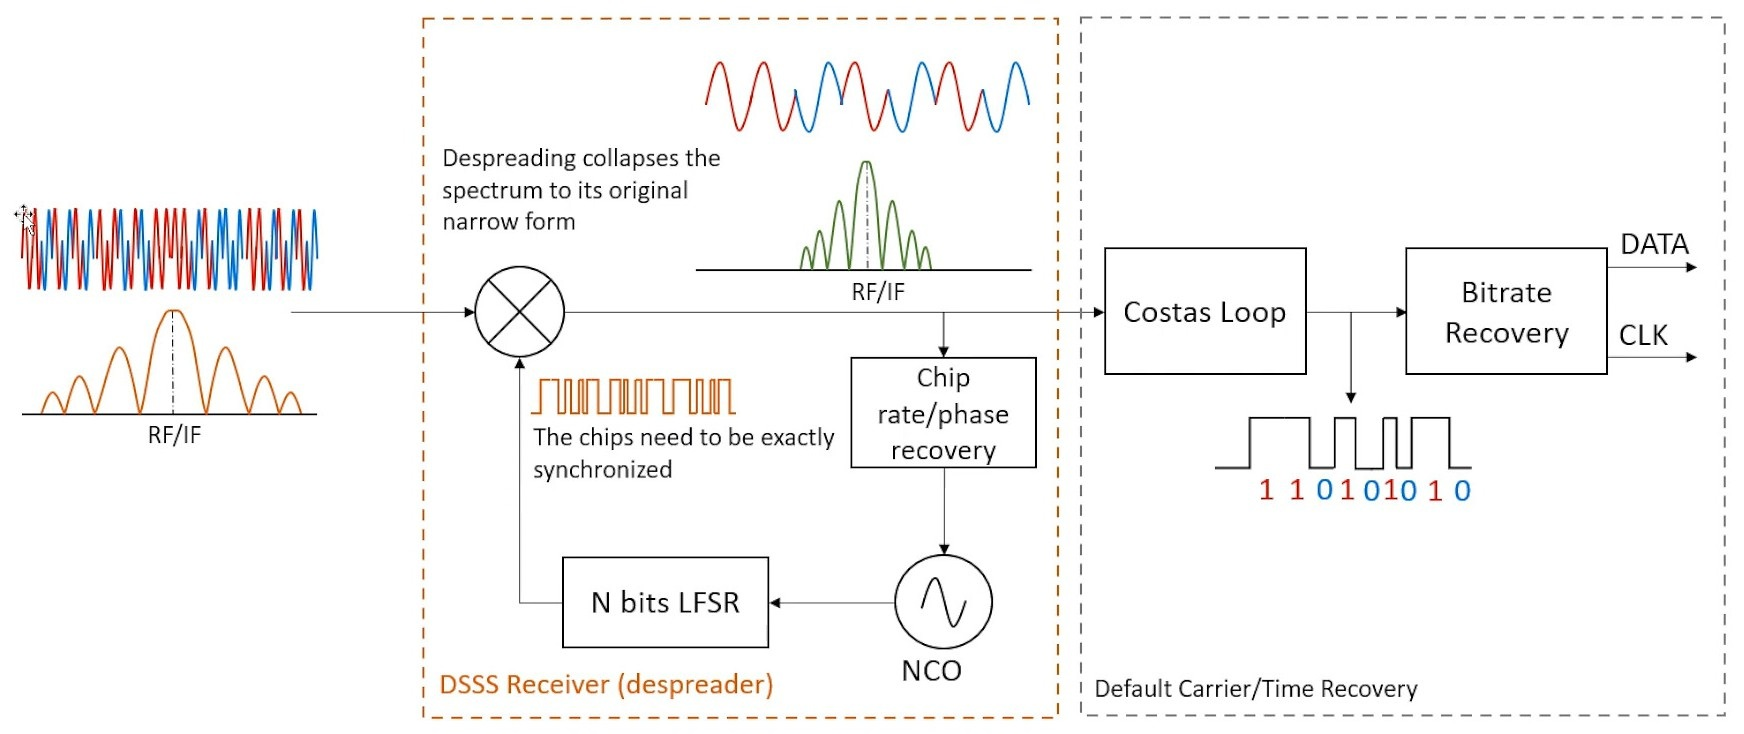
\includegraphics[scale = 0.3]{(845) Spread Spectrum Modulation and Demodulation - YouTube - 0-3-35.jpeg}
\end{figure}

\newpage 

\section{Tecniche a spettro espanso}
\footnote{Slide del prof | Spettro espanso | pag 1 \\
Appunti di Damiano | pag 1 \\ 
Slide | Spettro espanso | pag 1 \\
Appunti | 2025-05-06 | pag 5
} 


Un sistema a spettro espanso è realizzato sulla base di tecniche per cui il segnale trasmesso ha una occupazione spettrale 
maggiore (tra i $10^{3}$ ed i $10^{6}$ volte) di quella che avrebbe il convenzionale segnale modulato. \newline 

Di seguito le tre tecniche SS (Spread Spectrum) in cui si possono catalogare queste tecniche: 

\begin{itemize}
    \item FH-SS, cioè Frequency Hopping Spread Spectrum (principalmente utilizzato in ambito militare) 
    \item TH-SS, cioè Time Hopping Spread Spectrum 
    \item DS-SS, cioè Direct Sequence Spread Spectrum 
\end{itemize}

\newpage 

\subsection{Teorema di Shannon}
\footnote{Slide del prof | Spettro espanso | pag 2 - 4\\
Appunti di Damiano | pag 2 - 4\\ 
Slide | Spettro espanso | pag 2 - 4\\
Appunti | 2025-05-06 | pag 5 - 6
} 

Lo Spread Spectrum si basa sul teorema di Shannon. \newline 

Di seguita il teorema. \newline 

La capacità C, espressa in bps (cioè bit al secondo), 
di un canale AWGN è data da: 

{
    \Large 
    \begin{equation}
        \begin{split}
            C 
            &= 
            W 
            \cdot 
            \log_{2}
            \left(
                1 + \frac{S}{N_0 \cdot W}
            \right)
            \\
            &= 
            W 
            \cdot 
            \log_{2}
            \left(
                1 + \frac{S}{N}
            \right)
        \end{split} 
    \end{equation}
}

La capacità C fornisce la massima quantità di informazione che può essere trasmessa lungo il canale 
con probabilità di errore arbitrariamente piccola. \newline 

La capacità C è una funzione di W, cioè la banda in frequenza,  e il rapporto segnale-rumore $\frac{S}{N}$: 
quindi per aumentare C si deve aumentare la W, 
o aumentare il rapporto segnale rumore $\frac{S}{N}$, 
che a sua volta significa o aumentare il segnale S o diminuire il rumore N (cosa che è generalmente quasi impossibile fare). \newline

Grazie al teorema di Shannon, 
possiamo esprimere questa formula: 

{
    \Large 
    \begin{equation}
        \begin{split}
            C 
            &= 
            W 
            \cdot 
            \log_{2}
            \left(
                1 + \frac{S}{N}
            \right)
            \\
            &\downarrow
            \\
            \frac{C}{W}
            &=
            \log_{2}
            \left(
                1 + \frac{S}{N}
            \right)
            \\
            &= 
            1.44
            \ln
            \left(
                1 + \frac{S}{N}
            \right)
        \end{split}
    \end{equation}
}

Esprimere $\frac{C}{W}$ da una base 2 a una base e (che è appunto $\ln$), 
è molto comodo per i calcoli. \newline 

Quando: 

{
    \Large 
    \begin{equation}
        \frac{S}{N} \to 0
    \end{equation}
}

allora: 

{
    \Large 
    \begin{equation}
        \begin{split}
            \frac{C}{W}
            &=
            \log_{2}
            \left(
                1 + \frac{S}{N}
            \right)
            \\
            &\downarrow
            \\
            \frac{C}{W}
            &\approx
            1.44 \cdot \frac{S}{N} 
            \\
            &\downarrow
            \\
            W 
            &\approx 
            \frac{1}{1.44}
            \cdot 
            \frac{N}{S}
            \cdot 
            C
        \end{split}
    \end{equation}
}

Se C è finito, W tende a: 

{
    \Large 
    \begin{equation}
        W \to + \infty
    \end{equation}
}

Se W tende ad infinito significa che l'informazione è minore de rumore termico, 
quindi è più difficile capire se qualcuno sta trasmettendo 
perchè l'informazione sarà "nascosta" nel rumore. \newline 

\newpage 

\section{Vantaggi e modello base di un sistema SS }
\footnote{Slide del prof | Spettro espanso | pag 5 \\
Slide | Spettro espanso | pag 5 \\
Appunti | 2025-05-06 | pag 6 \\
Appunti | 2025-07-21 Ricevimento | pag 12.3
} 

"Spalmare" lo spettro del segnale originale comporta numerosi vantaggi. \newline 

Di seguito ne elenchiamo i principali: 

\begin{itemize}
    \item Protezione dall'interferenza 
    \item Spettri a bassa densità di potenza 
    \item Sicurezza nelle comunicazioni (negli anni c'è stato un cambio di paradigma riguardo all'uso dell'SS come metodo di sicurezza delle comunicazioni) 
    \item Messaggi "schermo" per chi cerca di spiare 
    \item Capacità di opporsi ad interferenze intenzionali (o il cosiddetto jamming)
    \item Il CDMA (Code Division Multiple Access) è una tecnica che sfrutta l'SS nella sua implementazione
\end{itemize}

\begin{tcolorbox}
Per messaggi schermo si intende chi intercetta il messaggio ha difficoltà a decifrato perchè è protetto da una lunga sequenza PN
\end{tcolorbox}

Di seguito un modello base di un sistema SS: 

\begin{figure}[h]
    \centering
    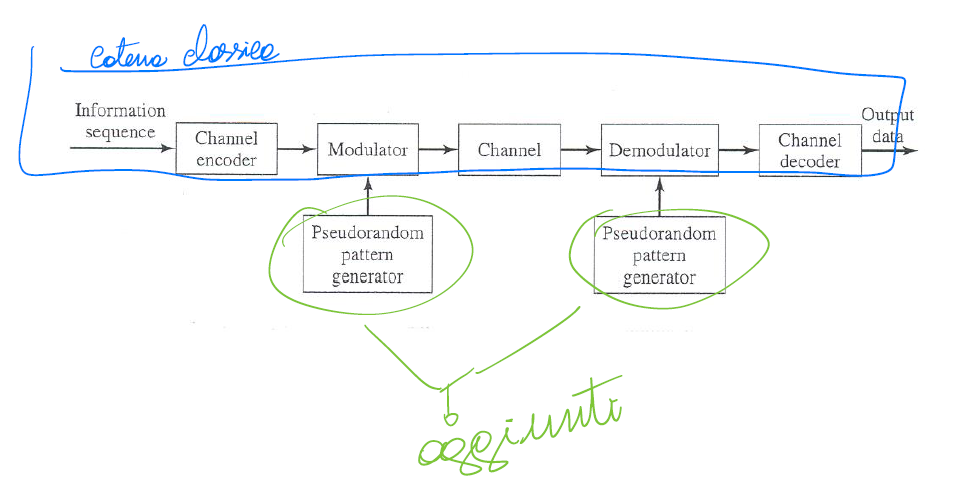
\includegraphics[scale = 0.8]{Modello base di un sistema SS con note.png}
\end{figure}

\newpage 

\section{Direct-Sequence Spread-Spectrum (DS-SS) }
\footnote{Slide del prof | Spettro espanso | pag 7 \\
Slide | Spettro espanso | pag 7 \\
Appunti | 2025-05-09 | pag 2
} 

Per applicare la DS-SS, 
viene applicata una modulazione in 2-PSK, 
la quale, come abbiamo studiato, 
ha una occupazione spettrale di banda di R: 

{
    \Large 
    \begin{equation}
        R = \frac{1}{T_b}
    \end{equation}
}

dove $T_b$ è il tempo di bit. \newline 

Siccome il modulatore, in un sistema SS, 
viene moltiplicato per una sequenza pseudo-casuale, 
la banda occupata con la tecnica DS-SS è di $B_c$:

{
    \Large 
    \begin{equation}
        B_c >> R
    \end{equation}
}

cioè, scritto per esteso, si intende che, il segnale DS-SS ha un'occupazione di banda molto larga. \newline

Questo accade perchè, al trasmettitore, la banda del segnale viene espansa fino a W:

{
    \Large 
    \begin{equation}
        W = B_c
    \end{equation}
}
utilizzando le sequenze PN (Pseudo-Noise). \newline 

\newpage 

\subsection{DS-SS: da bit rate a chip rate, formulazione matematica, e spreading }
\footnote{Slide del prof | Spettro espanso | pag 8 - 11\\
Appunti di Damiano | pag 9, 11 \\
Slide | Spettro espanso | pag 8 - 11\\
Appunti | 2025-05-09 | pag 2 - 4
} 

Riportando il modello base di un sistema SS: 

\begin{figure}[h]
    \centering
    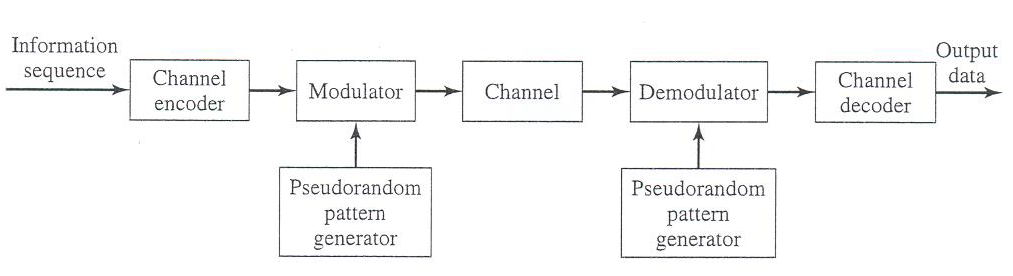
\includegraphics[scale = 0.8]{Modello base di un sistema SS senza note.png}
\end{figure}

notiamo che il modulatore moltiplica la sequenza informativa per la sequenza PN. \newline 

Per le formule matematiche che scriveremo di seguito, 
consideriamo: 

{
    \Large 
    \begin{equation}
        T_c << T_b
    \end{equation}
}

dove: 

\begin{itemize}
    \item $T_c$ viene definito come tempo di chip, cioè il tempo tra un'onda quadra e quella successiva nel segnale PN 
    \item $T_b$ viene definito come tempo di bit, che è il tempo del bit della sequenza informativa
\end{itemize}

Di seguito una figura dell'andamento dei segnali nel trasmettitore (con note): 

\begin{figure}[h]
    \centering
    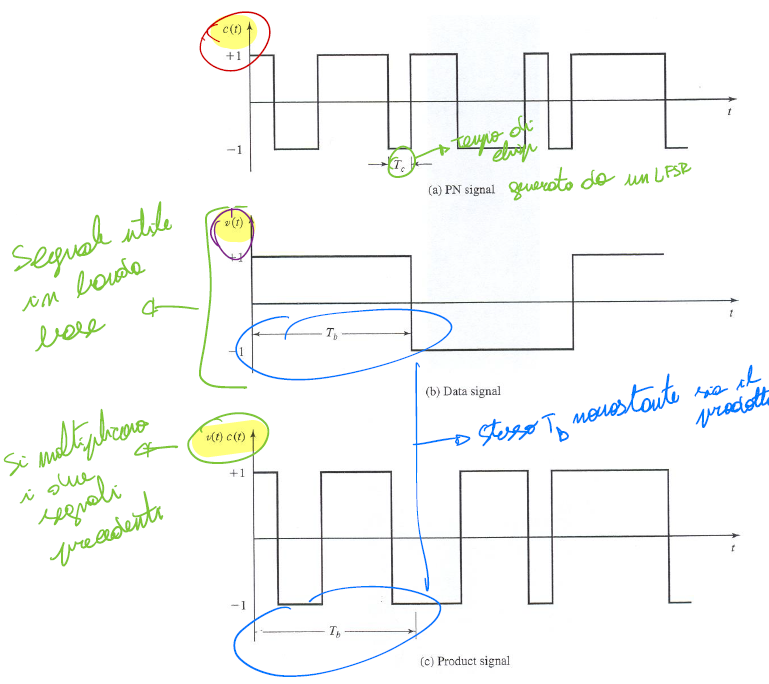
\includegraphics[scale = 0.8]{Andamenti di segnale nel trasmettitore in DS-SS.png}
\end{figure}

Possiamo esprimere il segnale dell'informazione v(t) come:

{
    \Large 
    \begin{equation}
    v(t) 
    = 
    \sum_{n = - \infty}^{+ \infty}
    a_n \cdot g_T(t - n \cdot T_b)       
    \end{equation}
}

dove: 

{
    \Large 
    \begin{equation}
        a_n = \pm 1
    \end{equation}
}

e $g_T$ è la funzione di base, dove, nei sistemi digitali, 
consideriamo degli impulsi rettangoli di periodo $T_b$. \newline 

\begin{tcolorbox}
    Matematicamente, 
    possiamo scrivere che l'andamento della sequenza PN va da $- \infty$ a $+ \infty$, 
    anche se, come abbiamo studiato nello scorso capitolo, un sistema reale elettronico non riesce ad elaborare infiniti elementi 
    e verranno divisi in N elementi, in cui N è un numero molto elevato
\end{tcolorbox}

Invece, possiamo esprimere il segnale PN come:

{
    \Large 
    \begin{equation}
    c(t) 
    = 
    \sum_{n = - \infty}^{+ \infty}
    c_n \cdot g_T(t - n \cdot T_b)       
    \end{equation}
}

dove: 

{
    \Large 
    \begin{equation}
        c_n = \pm 1
    \end{equation}
}

e $p$ è la funzione di PN da un LFSR. \newline 

Il modulatore moltiplica la portante con il segnale v(t) e il segnale c(t), 
e forma il segnale u(t), che si esprime come: 

{
    \Large 
    \begin{equation}
        \begin{split}
            u(t)
            &=
            \left[v(t) \cdot c(t)\right]
            \cdot 
            A_c \cdot \cos(2 \pi f_c t)
            \\
            &= 
            A_c \cdot \cos(2 \pi f_c t + \theta (t))
        \end{split}
    \end{equation}
}

dove: 
{
    \Large 
    \begin{equation}
        \theta(t) = v(t) \cdot c(t)
    \end{equation}
}

Alcune osservazioni riguardo l'espressione di u(t): 

\begin{itemize}
    \item si fa una modulazione per traslare $v(t) \cdot c(t)$ alla frequenza $f_c$
    \item se v(t) e c(t) sono impulsi rettangolari, quindi il prodotto può valere solo 1 o 0
\end{itemize}

\newpage 

In frequenza possiamo confrontare i segnale v(t), c(f) e u(t) con questo figura: 

\begin{figure}[h]
    \centering
    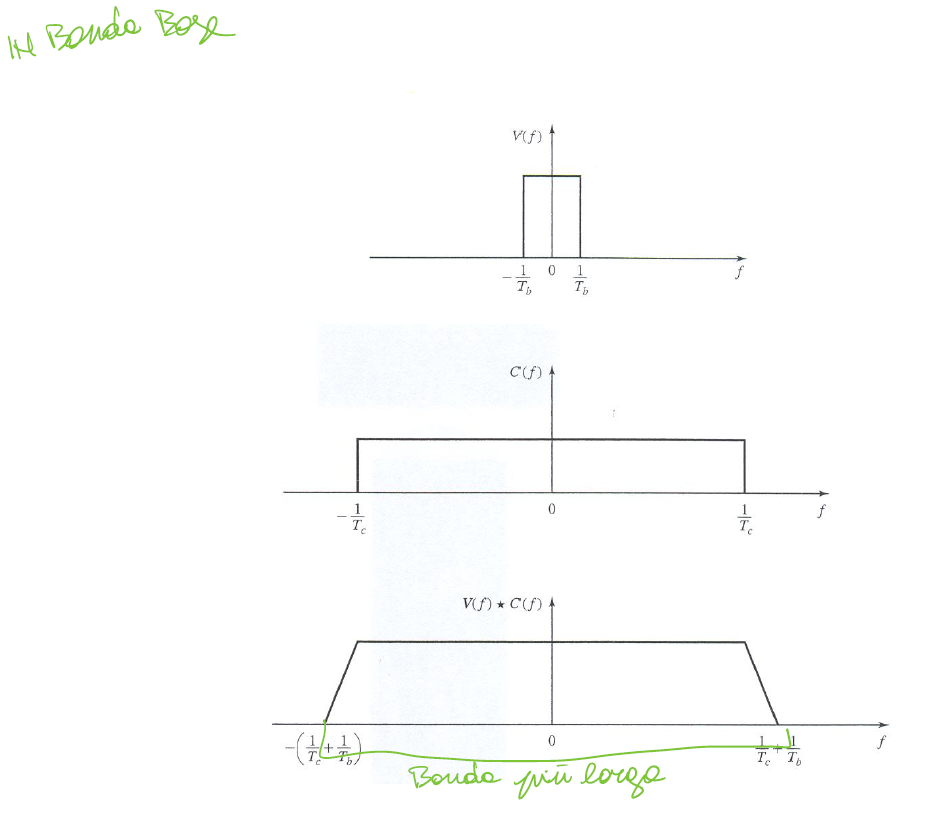
\includegraphics[scale = 0.7]{Spreading visualizzato DS-SS.png}
\end{figure}

Altre osservazione osservando questo grafico: 

\begin{itemize}
    \item non per forza i segnali devono essere rettangolari: vengono usati per comodità grafiche 
    \item l'espansione della banda da $\frac{1}{T_b}$ diventa $\frac{1}{T_c} + \frac{1}{T_b}$, quindi la banda viene aumentata dalle $10^{3}$ alle $10^{6}$ volte 
    \item il canale, per non avere distorsione, deve avere la banda disponibile 
    \item Siccome si fa una moltiplicazione nel tempo, grazie alle proprietà tra tempo e frequenza, in frequenza avviene una convoluzione tra V(f) e C(f), che sono rispettivamente v(t) e c(t) in frequenza
\end{itemize}

\newpage 

\subsection{DS-SS: despreading, demodulazione e interferenze a banda stretta }
\footnote{Slide del prof | Spettro espanso | pag 12 - 13\\
Slide | Spettro espanso | pag 12 - 13 \\
Appunti | 2025-05-09 | pag 5
} 

Quando si de-modula in digitale, 
il primo step è la sincronizzazione, 
perchè in digitale, se non si ha una sincronizzazione, 
si ricevono sequenze che non hanno senso. \newline 

Il rumore, in particolare, cambia i valori. \newline 

Di seguito lo schema di un demodulatore che fa anche da despreading: 

\begin{figure}[h]
    \centering
    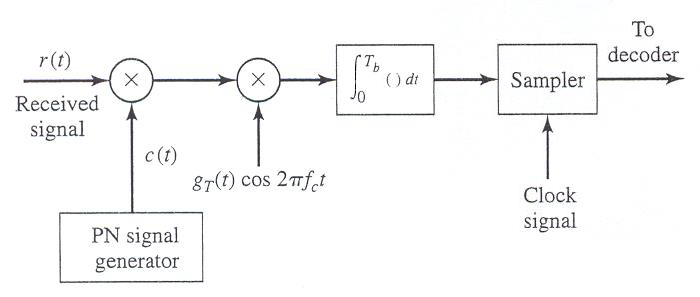
\includegraphics[scale = 0.8]{DS-SS Modello Despreading e demodulatore.png}
\end{figure}

Ricordando la formula di r(t), per adesso senza rumore,
cioè il segnale trasmesso: 

{
    \Large 
    \begin{equation}
        r(t)
        =
       \left[v(t) \cdot c(t)\right]
            \cdot 
            A_c \cdot \cos(2 \pi f_c t)
    \end{equation}
}

Se c'è perfetta sincronizzazione, 
la fase in ricezione e in trasmissione è 
la stessa. \newline 

Quindi possiamo porre in ricezione: 

{
    \Large 
    \begin{equation}
        \theta (t) = 0
    \end{equation}
}

Se moltiplichiamo r(t) per una sequenza PN c(t), 
possiamo esprimere la formula del segnale in despreding: 

{
    \Large 
    \begin{equation}
        \begin{split}
            r(t) \cdot c(t)
            &= 
            \{
            \left[v(t) \cdot c(t)\right]
            \cdot 
            A_c \cdot \cos(2 \pi f_c t)
            \}
            \cdot
            c(t)
            \\
            &= 
            A_c \cdot v(t) \cdot c^{2} (t) \cos(2 \pi f_c t)
            \\
            &= 
            A_c \cdot v(t) \cdot \cos(2 \pi f_c t)
        \end{split}
    \end{equation}
}

Ma, se consideriamo l'interferenza i(t), 
il segnale r(t) ricevuto non è quello scritto precedente, 
ma diventa: 

{
    \Large 
    \begin{equation}
        r(t)
        =
        \left[v(t) \cdot c(t)\right]
        \cdot 
        A_c \cdot \cos(2 \pi f_c t) + i(t)
    \end{equation}
}

Quindi, se consideriamo il despreding, se si moltiplica r(t) per c(t) 
non è quello precedente del caso ideale, bensì: 

{
    \Large 
    \begin{equation}
            r(t) \cdot c(t)
            = 
            \left[A_c \cdot \cos(2 \pi f_c t) \right]
            + 
            \left[i(t) \cdot c(t)\right]
    \end{equation}
} 

La prima parte della equazione tra parentesi quadre, 
cioè $A_c \cdot \cos(2 \pi f_c t)$ è voluta, 
invece $i(t) \cdot c(t)$ non è voluta, è indesiderata. \newline 

L'operazione di despreading trasforma il segnale a banda stretta del disturbo i(t), 
in segnale banda larga perchè i(t) è banda stretta e viene moltiplicato per c(t), 
che è a banda larga. \newline 

Solo una frazione di $\frac{R}{W}$ (che per noi, in digitale è il rapporto segnale-rumore) 
della potenza interferente disturba il segnale utile. \newline 

Considerando l'interferenza ideale i(t): 

{
    \Large 
    \begin{equation}
        i(t)
        = 
        A_l \cdot \cos(2 \pi f_I t)
    \end{equation}
}

dove: 

\begin{itemize}
    \item $A_l$ è l'ampiezza del disturbo i(t)
    \item $f_I$ è la frequenza in cui si trova il disturbo a banda stretta i(t)
\end{itemize}

Sapendo che, il disturbo i(t) è ergodico, stazionario e bilatero, 
possiamo scrivere che, 
la potenza del rumore i(t) vale: 

{
    \Large 
    \begin{equation} 
        P_I 
        = 
        \frac{(A_I)^{2}}{2}    
    \end{equation}
}

La densità spettrale di potenziale dell'interferente, 
dopo il despreading, vale: 

{
    \Large 
    \begin{equation}
        I_0 
        =
        \frac{P_I}{W}
    \end{equation}
}

dove W è la banda del canale. \newline 

La potenza interferente all'uscita del demodulatore vale: 

{
    \Large 
    \begin{equation}
        \begin{split}
            I_0 \cdot R 
            &=
            P_I \cdot \frac{R}{W}
            \\
            &= 
            \frac{P_I}{W / R}
        \end{split}
    \end{equation}
}

Quindi, la potenza interferente all'uscita del demodulatore dipende dal rapporto $\frac{W}{R}$: 
più $\frac{W}{R}$ è grande, e più $\frac{P_I}{W / R}$ diminuisce e viceversa. \newline 

\newpage 

\section{Guadagno di processo (Process Gain)}
\footnote{Slide del prof | Spettro espanso | pag 14 \\
Slide | Spettro espanso | pag 14 \\
Appunti | 2025-05-09 | pag 5
} 

Per guadagno di processo si intende di quando aumenta la banda in SS dalla banda originale. \newline 

Se consideriamo $L_C$ il guadagno di processo, 
possiamo esprimerlo come: 

{
    \Large 
    \begin{equation}
        L_C = \frac{W}{R} = \frac{T_b}{T_c}
    \end{equation}
}

dove: 

\begin{itemize}
    \item $T_b$ è il tempo di bit 
    \item $T_c$ è il tempo di chip, cioè il periodo di un bit della sequenza Pseudo-Noise
\end{itemize}

Esprimere il rapporto tra i rapporti dei segnali rumori tra il segnale SS e quello con interferenza dentro all'SS, 
possiamo scriverla come: 

{
    \Large 
    \begin{equation}
        \frac{\left( \frac{S}{N} \right)_o}{\left( \frac{S}{N} \right)_i}
    \end{equation}
}

dove: 

\begin{itemize}
    \item $\left( \frac{S}{N} \right)_o$ è il rapporto segnale rumore con SS 
    \item $\left( \frac{S}{N} \right)_i$ è il rapporto segnale rumore con rumore con SS
\end{itemize}

applicando le proprietà dei dB, 
la frazione diventa una sottrazione, cioè: 

{
    \Large 
    \begin{equation}
        \frac{\left( \frac{S}{N} \right)_o}{\left( \frac{S}{N} \right)_i} 
        \to 
        \left.
        \left( \frac{S}{N} \right)_o 
        \right|_{dB}
        - 
        \left.
        \left( \frac{S}{N} \right)_i 
        \right|_{dB}
    \end{equation}
}

Nelle SS, generalmente $  \left. \left( \frac{S}{N} \right)_i \right|_{dB}$ è molto basso: 
ecco perchè si preferisce utilizzare le tecniche SS. \newline 

La riduzione della potenza interferente, storicamente, 
è il primo motivo che ha condotto all'introduzione dei sistemi SS, 
migliorando le prestazioni in canali affetta da interferenza. \newline 

\begin{tcolorbox}
Un esempio pratico di come è molto utile una SS è proprio quella impiegata nella trasmissione Wi-Fi. \newline 

Ti consiglio questo video sul Wi-Fi 7 e di come venga gestito lo spettro in caso di interferenze: \newline 

\url{https://www.youtube.com/watch?v=D_1qfsdOmJU}\\
Arriva il Wi-Fi 7 in Italia: come funziona il nuovo standard portato da Iliad by Stefano Bolis \newline 

Per un maggior approfondimento, 
in particolare riguardo alla tecnica Puncturing per evitare le bande occupate da altri utenti o dovute alle interferenze, 
ti lascio il sito della intel dove ne discute in modo approfondito: \newline 

\url{https://www.intel.com/content/www/us/en/products/docs/wireless/wi-fi-7.html}

\end{tcolorbox}

\newpage 

\section{Ruolo delle sequenze PN}
\footnote{Slide del prof | Spettro espanso | pag 15 \\
Appunti di Damiano | pag 15 \\ 
Slide | Spettro espanso | pag 15 \\
Appunti | 2025-05-09 | pag 5
} 

La sequenza Pseudo-Noise (o chiamata anche sequenza dei coefficienti $\{  C_n \}$) 
è nota solo al ricevitore autorizzato: 
questo è un primo livello di protezione dato dall'SS con LFSR. \newline 

Un ricevitore che non conosce la sequenza PN, 
non può de-modulare correttamente l'informazione. \newline 

L'uso della sequenza PN fornisce un primo livello di sicurezza, 
che non è possibile con le modulazioni convenzionali. \newline 

\begin{tcolorbox}
    La sequenza di coefficienti $\{ C_n\}$ è come la chiave di una porta: 
    se ce l'hai, puoi entrare nella stanza, se non ce l'hai, non entri. \newline 

    Per adesso consideriamo il caso ideale, 
    anche se sai già bene che questa caratteristica non è del tutto vero perchè abbiamo a che fare con LFSR, 
    i quali implementano degli algoritmi, e quindi deterministici e non del tutto realmente casuali
\end{tcolorbox}

Ma (in ingegneria c'è sempre un ma) il costo del miglioramento ottenuto è, 
oltre all'allagamento della banda, 
un incremento della complessità del sistema. \newline 

\begin{tcolorbox}
    
    Da \url{https://www.youtube.com/watch?v=EkX_O0AaSI0} \\
    La spada nella roccia: "Questo il mondo far girar" \newline    
    
    Questo il mondo fa girar \\
    per ogni qua c'è sempre un là\\
    per ogni se "c'è sempre un ma"\\
    per ogni su "c'è sempre un giù"\\
    per ogni meh "c'è sempre un più"
\end{tcolorbox}

\newpage 

\section{Probabilità di errore in ricezione}
\footnote{Slide del prof | Spettro espanso | pag 16 - 19\\
Appunti di Damiano | pag 17 - 18\\ 
Slide | Spettro espanso | pag 16 - 19 \\
Appunti | 2025-05-09 | pag 5 - 6
} 

\begin{tcolorbox}
Come sempre, l'importante sono le considerazioni e non le formule per la teoria    
\end{tcolorbox}

In questo caso, nella SS, 
non consideriamo il rumore termico. \newline 

Consideriamo solo un segnale indesiderato interferente sovrapposto, 
che abbrevieremo con la dicitura interferente. \newline 

L'interferente influisce e aumenta la probabilità di errore del segnale in ricezione r(t). \newline 

Consideriamo questo schema per un ricevitore SS: 

\begin{figure}[h]
    \centering
    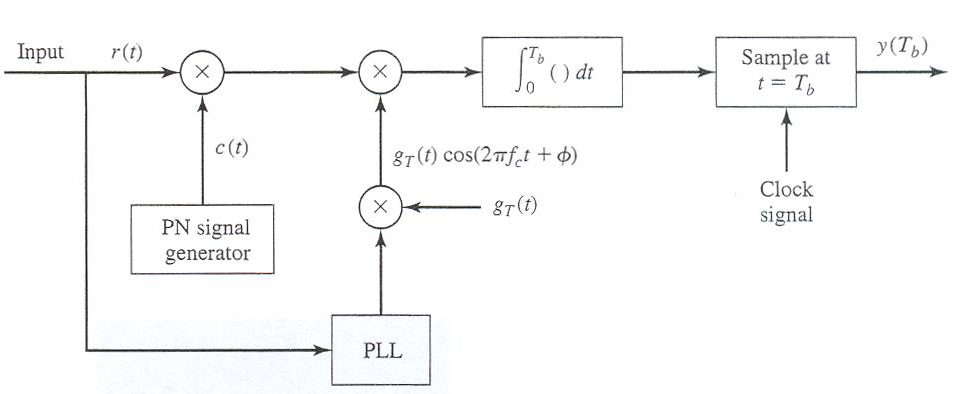
\includegraphics[scale = 0.7]{Ricevitore SS con inteferente.png}
\end{figure}

Consideriamo il segnale il segnale prima dell'integratore s(t) come: 

{
    \Large 
    \begin{equation}
        s(t)
        = 
        a_0 
        \cdot 
        g_T(t)
        \cdot 
        c(t)
        \cdot 
        \cos(2 \pi f_c t)
    \end{equation}
}

dove: 

{
    \Large 
    \begin{equation}
        a_0 = \pm 1
    \end{equation}
}

perchè è una sequenza digitale, 
si pone non solo $a_0 = \pm 1$, 
ma anche la funzione di base ha la seguente funzione di base:  

{
    \Large 
    \begin{equation}
        g_T (t)
        = 
        \begin{cases}
            \sqrt{\frac{2 \cdot E_b}{T_b}}
            \text{ per }
            0 \le t \le T_b 
            \\
            0 
            \text{ altrove}
        \end{cases}
    \end{equation}
}

e inoltre manca anche la formulazione matematica della sequenza Pseudo-Noise 
c(t), che vale: 

{
    \Large 
    \begin{equation}
        c(t)
        =
        \sum_{n = 0}^{L_c - 1}
        c_n \cdot p(t - n \cdot T_c)
    \end{equation}
}

In quanto la sequenza $\{ c_n \}$ si può assumere incorrelata, 
allora l'energia tra il prodotto dei $\{ c_n\}$ in ricezione 
e il prodotto dei $\{ c_m\}$ coefficienti generati dal ricevitore vale: 

{
    \Large 
    \begin{equation}
        E(c_n \cdot c_m)
        \approx 
        E(c_n)
        \cdot 
        E(c_m)
    \end{equation}
}

Sapendo che il singolo valore $c_n$ appartiene a questo intervallo: 

{
    \Large 
    \begin{equation}
        c_n \in [-1, +1]
    \end{equation}
}

e ogni $c_n$ della sequenza $\{ c_n\}$ è equiprobabile, 
allora l'energia di ogni $c_n$ vale: 

{
    \Large 
    \begin{equation}
        E (c_n)
        = 
        0
    \end{equation}
}

In altre parole, 
il valore medio di $c_n$ nel periodo $T_b$ è uguale a zero. \newline 

Invece l'energia del valore quadratico medio di ogni elemento di $c_n$, 
vale: 

{
    \Large 
    \begin{equation}
        E(c_n^{2})
        = 
        1
    \end{equation}
}

Considerano il segnale in uscita, 
quindi dopo l'integratore e il campionatore, 
avremo $y_I (T_b)$ che vale: 

{
    \Large 
    \begin{equation}
        \begin{split}
            y_I (T_b)
            &=
            \int_{0}^{T_b}
            c(t) 
            \cdot
            g_T (t)
            \cos(2 \pi f_c t + \theta)
            \cdot 
            i(t)
            dt
            \\
            &=
            \int_{0}^{T_b}
            \sum_{n = 0}^{L_c - 1}
            c_n
            \cdot
            p(t - n \cdot T_c)
            \cdot
            \sqrt{\frac{2 \cdot E_b}{T_b}}
            \cdot 
            \cos(2 \pi f_c t + \theta)
            \cdot 
            i(t)
            dt
            \\
            &=  
            \sqrt{\frac{2 \cdot E_b}{T_b}}
            \cdot
            \sum_{n = 0}^{L_c - 1}
            c_n
            \cdot 
            \int_{0}^{T_b}
            p(t - n \cdot T_c)
            \cdot 
            i(t)
            \cdot 
            \cos(2 \pi f_c t + \theta)
            dt
        \end{split}
    \end{equation}
}

A questo punto, sapendo che: 

{
    \Large 
    \begin{equation}
        T_c << T_b
    \end{equation}
}

cioè il tempo di chip $T_c$ della PN è molto minore del tempo di bit $T_b$, 
allora possiamo svolgere l'integrale non nell'intervallo $[0, T_b]$, 
bensì nell'intervallo $[n \cdot T_c, (n+1) \cdot T_c]$, cioè tra due periodi di $T_c$. \newline 

Inoltre, sappiamo che, dalle sequenze PN con LFSR: 

{
    \Large 
    \begin{equation}
        p(t - n \cdot T_c) \neq 0
    \end{equation}
}

in un periodo multiplo di $T_c$. \newline 

Con queste osservazioni, 
possiamo riscrivere la formula di $y_I (T_b)$ come: 


{
    \Large 
    \begin{equation}
        \begin{split}
        y_I (T_b)
        &=
        \sqrt{\frac{2 \cdot E_b}{T_b}}
            \cdot
            \sum_{n = 0}^{L_c - 1}
            c_n
            \cdot 
            \int_{0}^{T_b}
            p(t - n \cdot T_c)
            \cdot 
            i(t)
            \cdot 
            \cos(2 \pi f_c t + \theta)
            dt
        \\
        &\downarrow
        \\
        y_I (T_b)
        &=
        \sqrt{\frac{2 \cdot E_b}{T_b}}
            \cdot
            \sum_{n = 0}^{L_c - 1}
            c_n
            \cdot 
            \int_{n \cdot T_c}^{(n+1) \cdot T_c}
            i(t)
            \cdot 
            \cos(2 \pi f_c t + \theta)
            dt
            \\
            &= 
              \sqrt{\frac{2 \cdot E_b}{T_b}}
            \cdot
            \sum_{n = 0}^{L_c - 1}
            c_n
            \cdot
            v_n
        \end{split}
    \end{equation}
}

Possiamo scrivere: 

{
    \Large 
    \begin{equation}
        v_n = 
        \int_{n \cdot T_c}^{(n+1) \cdot T_c}
            i(t)
            \cdot 
            \cos(2 \pi f_c t + \theta)
            dt
    \end{equation}
}

Grazie al teorema del limite centrale per $L_c$ molto elevato, 
si può approssimare la sommatoria ad una gaussiana . \newline 

\newpage 

\subsection{Interferente monocromatico}
\footnote{Slide del prof | Spettro espanso | pag 20 \\
Slide | Spettro espanso | pag 20 
} 

Se consideriamo interferenza monocromatica del tipo:

{
    \Large 
    \begin{equation}
        i (t)
        = 
        \sqrt{2 \cdot P_I}
        \cdot 
        \cos(2 \pi f_c t + \varTheta_I )
    \end{equation}
}

e consideriamo $\varTheta_I$ una variabile aleatoria uniformemente distribuita tra: 

{
    \Large 
    \begin{equation}
        \varTheta_I \in [0, 2\pi]
    \end{equation}
}

Allora possiamo esprimere la probabilità di errore sul bit in una DS-SS in ricezione come: 

{
    \Large 
    \begin{equation}
        P_{Eb} 
        = 
        \left(
            \sqrt{\frac{2 \cdot E_b}{I_0}}
        \right)
    \end{equation}
}

dove con la funzione Q si intende la funzione erfc della gaussiana. \newline 

\begin{tcolorbox}
    Ricordati di utilizzare e di portare all'esame le tabelle dell'erfc
\end{tcolorbox}

\newpage 

\subsection{Interference margin}
\footnote{Slide del prof | Spettro espanso | pag 21 \\
Appunti di Damiano | pag 21 \\
Slide | Spettro espanso | pag 21 
} 

Consideriamo che il rapporto tra l'energia del bit $E_b$ e la potenza del rumore $I_0$ sul bit vale:

{
    \Large 
    \begin{equation}
            \frac{E_b}{I_0}
            =
            \frac{P_S \cdot T_b}{\frac{P_I}{W}}
            = 
            \frac{\frac{P_S}{R}}{\frac{P_I}{W}}
            = 
            \frac{\frac{W}{R}}{\frac{P_I}{P_S}}
            =
            \frac{L_C}{\frac{P_I}{P_S}}
    \end{equation}
}

e quindi: 

{
    \Large 
    \begin{equation}
        \frac{E_b}{I_0}
        =  
        \frac{L_C}{\frac{P_I}{P_S}}
    \end{equation}
}

dove: 

\begin{itemize}
    \item $E_b$ è l'energia sul bit 
    \item $I_0$ è l'energia dell'interferente sul bit
    \item $P_S$ è la potenza del segnale con SS
    \item $T_b$ è il tempo di bit 
    \item $P_I$ è la potenza dell'interferente 
    \item W è la banda del segnale 
    \item R è il rate
    \item $L_C$ è il guadagno di processo dovuto alla SS 
\end{itemize}

Allora in dB possiamo scrivere: 

{
    \Large 
    \begin{equation}
        \left( \frac{P_I}{P_S}\right)_{dB}
        = 
        \left(L_C\right)_{dB}
        - 
        \left(\frac{E_b}{I_0}\right)_{dB}
    \end{equation}
}

$\frac{P_I}{P_S}$ prende il nome di Interference margin. \newline 

\newpage 

\subsubsection{Interference margin: esempio numerico}
\footnote{Slide del prof | Spettro espanso | pag 21 \\
Appunti di Damiano | pag 21 \\
Slide | Spettro espanso | pag 21 
} 


Considerando i seguenti dati: 

{
    \Large 
    \begin{equation}
        \begin{cases}
            \left(\frac{E_b}{I_0}\right)_{dB}
            = 
            10 dB 
            \\
            \left(\frac{P_I}{P_S}\right)_{dB}
            = 
            20 dB 
        \end{cases}
    \end{equation}
}

dove $\frac{E_b}{I_0}$ è il rapporto segnale-rumore senza SS, 
allora abbiamo bisogno di un $L_C$ in dB che vale: 

{
    \Large 
    \begin{equation}
        \left(L_C\right)_{dB} = 30 \text{ dB}
    \end{equation}
}

che in un numeri non logaritmici vale: 

{
    \Large 
    \begin{equation}
        \begin{split}
            \left(L_C\right)_{dB} &= 30 \text{ dB}
            \\
            &\downarrow
            \\
            \frac{W}{R} &= 1000
        \end{split}
    \end{equation}
}

Questo significa che la potenza dell'interferente può essere 1000 volte maggiore della potenza del segnale utile, 
ma, grazie all'SS, 
si può mantenere la qualità desiderata. \newline 

\newpage 

\subsection{Interferente a banda larga}
\footnote{Slide del prof | Spettro espanso | pag 22 - 23\\
Slide | Spettro espanso | pag 22 - 23 \\
Appunti | 2025-07-21 Ricevimento | pag 13
} 

Rispetto al caso monocromatico precedente, 
consideriamo adesso un interferente a banda larga come nella seguente figura: 

\begin{figure}[h]
    \centering
    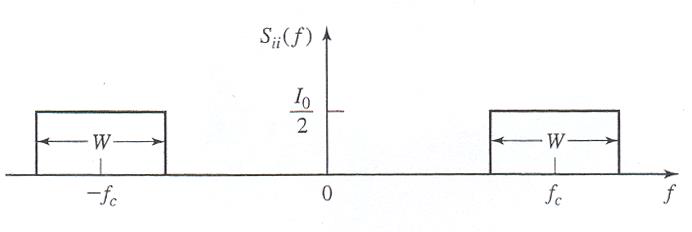
\includegraphics[scale = 1]{Interferente a banda larga.png}
\end{figure}

\begin{tcolorbox}
    Senza dimostrazione, formule che ci dovete credere come un dogma. 
\end{tcolorbox}

La probabilità di errore sul bit considerando una interferente a banda larga come in figura, 
vale: 

{
    \Large 
    \begin{equation}
        P_{Eb}
        = 
        Q
        \left(
            \frac{2 \cdot E_b}{I_0 \cdot J(\alpha)}
        \right)
    \end{equation}
}


dove: 

{
    \Large 
    \begin{equation}
        J(\alpha)
        =
        2 \cdot 
        \int_{0}^{+ \infty}
        \left(
            1 - \frac{x}{\alpha}
        \right)
        \cdot 
        \frac{\sin(pi \cdot x)}{pi \cdot x}
        dx
    \end{equation}
}

dove a sua volta: 

{
    \Large 
    \begin{equation}
        \alpha = W \cdot T_c
    \end{equation}
}

\newpage 

Generalmente non calcoliamo questo integrale, 
ma, come spesso accade, utilizziamo i grafici. \newline

Possiamo tracciare l'andamento di $J(\alpha)$ come: 

\begin{figure}[h]
    \centering
    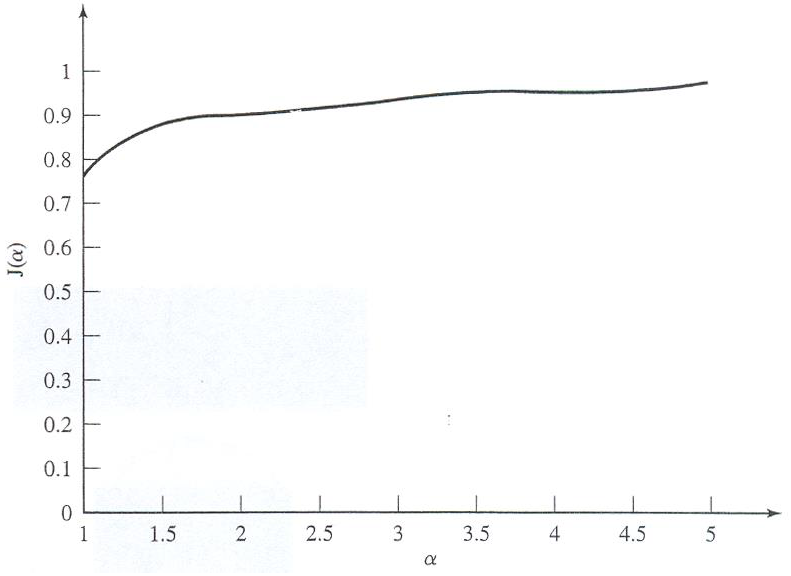
\includegraphics[scale = 0.7]{Andamento di J alpha.png}
\end{figure}

La probabilità di errore con la interferente a banda larga è minore 
rispetto all'esempio della banda mono-cromatica. \newline 

\newpage 

\section{DS-SS: applicazioni}
\footnote{Slide del prof | Spettro espanso | pag 24 \\
Slide | Spettro espanso | pag 24 \\
Appunti | 2025-05-13 | pag 2 
} 

\begin{tcolorbox}
    Il prof scrive le applicazioni del DS-SS in Inglese (cosa buona e giusta), 
    però qui proverò a dare una traduzione in italiano perchè so che l'inglese non è il vostro forte. \newline

    Utilizzo questa occasione per ricordare di studiare e parlare l'inglese bene, 
    non a livello madrelingua, ma almeno bene. \newline 

    Sulla rete ci sono taaaanti materiali: da video a podcast, a dirette su Twitch a libri. Tutto. \newline 

    Per piacere, usufruitene
\end{tcolorbox}


Di seguito delle applicazioni del DS-SS: 

\begin{itemize}
    \item Trasmissioni di segnale a basso rilevabilità (Low-detectability signal trasmission)
    \item Accesso multiplo a divisione di codice (Code Division Multiple Access o CDMA) 
    \item Comunicazioni in canali con percorso multipli (Communication over channel with multipath)
\end{itemize}

\begin{tcolorbox}
    I percorsi multipli li avevamo già visti nel precedente corso. \newline 

    Un breve ripasso da Tds: \\
    \url{https://github.com/ciccio25/appunti-teoria-dei-segnali/blob/main/Appunti%20Teoria%20dei%20segnali.pdf} \\
    Capitolo 5.3.3 - Distorsione causata da percorsi multipli - pag 50 - 51 \newline 

    I multipath sono alla base delle comunicazioni moderne: basti pensare alla tecnica MI-MO (Multiple Input, Multiple Output) 
    del Wi-Fi o del 5G. \newline 

    Un esempio in questo video: \newline 

    \url{https://youtu.be/e9x5PANDAuU?si=FdVu5UgL0YWPbdBY} \\
    MU-MIMO nelle reti Wi-Fi: come funziona, perchè è importante e potenzialità con il Wi-Fi 6 by Stefano Bolis \newline 

    Invece per visualizzare il concetto da un punto di vista generale: \newline 

    \begin{itemize}
        \item \url{https://www.youtube.com/watch?v=B2h8FohnwUs} \\ MU-MIMO Explained by PowerCert Animated Videos 
        \item \url{https://youtu.be/0ncIWlhsu1A?si=2txuVFDsNfOhYnXA} \\ What is Multi-User MIMO Communications (MU MIMO)? by Iain Explains Signals, Systems, and Digital Comms
    \end{itemize}

\end{tcolorbox}


\newpage 

\subsection{Low detectability signal trasmission}
\footnote{Slide del prof | Spettro espanso | pag 25 \\
Slide | Spettro espanso | pag 25 \\
Appunti | 2025-05-13 | pag 2 
} 

Il segnale utile è trasmesso con un livello di potenza molto basso (confrontabile con il rumore). \newline 

Sapendo che la potenza del rumore $P_N$ vale: 

{
    \Large 
    \begin{equation}
        P_N 
        = 
        W \cdot N_0
    \end{equation}
}

dove: 

\begin{itemize}
    \item W è banda che consideriamo 
    \item $N_0$ è il rumore
\end{itemize}

Se consideriamo $P_R$ la potenza del segnale in ricezione, 
possiamo compararla con la potenza del rumore $P_N$: 

{
    \Large 
    \begin{equation}
        \frac{P_R}{P_N}
        <<
        1
    \end{equation}
}

cioè, come scritto precedentemente, 
il segnale utile ha un livello di potenza molto basso. \newline 

Un ricevitore autorizzato, e che ha quindi i famosi coefficienti $\{ c_n\}$ dell'LFSR Pseudo-Noise, 
può recuperare l'informazione, 
con qualità soddisfacente, utilizzando il processo di despreading. \newline 

Invece, il ricevitore non autorizzato non può conseguire il necessario miglioramento del rapporto segnale-rumore. \newline 

Quindi, con il DS-SS si ha una bassa probabilità di intercettazione. \newline 

Possiamo considerare il segnale con DS-SS, grazie a questa proprietà, 
come segnale LPI (Low Probability of Intercept). \newline 

\newpage 

\subsection{CDMA}
\footnote{Slide del prof | Spettro espanso | pag 28 - 29\\
Appunti di Damiano | pag 28 - 29\\
Appunti | 2025-05-13 | pag 3 
} 

Il guadagno di processo $L_C$ può essere utilizzato per consentire la trasmissione 
simultanea di segnali provenienti da utenti diversi (e sovrapposti nel tempo e in frequenza). \newline 

\begin{tcolorbox}
    Il caso delle comunicazioni moderne, specialmente quelle senza filo, 
    è come entrare in una stanza piena di persone, dove si sta stretti, 
    ognuno parla ad alta voce e tu sei lì che devi capire la persona che ti sta davanti o dall'altra parte della stanza. \newline 

    Nella realtà o scappi dalla stanza o cerchi il possibile di farti capire con le gesta (come un vero italiano stereotipato). \newline 

    Nelle tecnologie moderne SS, questo "casino" è intenzione e inoltre è possibile, 
    se si è autorizzati, capire qualsiasi persona nella stanza
\end{tcolorbox}

Ciascun utente deve essere identificato da una diversa sequenza Pseudo-Noise, 
chiamata firma (o signature in inglese). \newline 

Le sequenze PN devono essere scelte in modo da avere buone proprietà di correlazione 
(quindi auto-correlazione e cross-correlazione). \newline 

\begin{tcolorbox}
    Ricordo al volo che la correlazione è diversa dalla auto-correlazione, 
    che a sua volta è diversa dalla correlazione mutua
\end{tcolorbox}

Al ricevitore, 
i segnali con sequenza di codice diversa da quella di interesse 
appaiono come segnali interferenti. \newline 

L'entità dell'interferenza dipende principalmente dalle seguenti caratteristiche: 

\begin{itemize}
    \item dal numero di utenti 
    \item dalle proprietà di cross-correlazione delle sequenze scelte
\end{itemize}

Il grosso vantaggio del CDMA rispetto agli altri schemi di multiplazione è la flessibilità. \newline 

\newpage 

\begin{tcolorbox}
    In altri casi, ad esempio la FDM (Frequency Division Multiplexing), 
    per aggiungere un altro trasmettitore, bisogna ridividere in parti uguali la banda assegnata W. \newline 

    Invece nella CDMA ho un numero massimo di firme PN. \newline 

    Finché un trasmettitore trasmette, avrà la sua firma, 
    quando non trasmetterà quella stessa firma verrà assegnata ad un altro utente, 
    così da non aumentare il disturbo dovuto agli altri segnali e/o utenti nello spettro. \newline 

    È ovvio che, nelle tecniche di trasmissione moderne, si utilizza il CDMA insieme ad altre tecniche di modulazione, 
    in questo caso di esempio CDMA-FDM, oppure CDMA-TDM e così via

    Piccola parentesi storica: 
    l'azienda Qualcoom ha spinto tanto, 
    quando introdusse l'UMTS/GSM (o anche chiamata dagli operatori "Great Source of Money"), 
    quello che comunemente chiamavamo 3G, 
    sul CDMA. \newline 

    Un po' di storia di quello che era successo ai tempi: \newline 

    \url{https://www.youtube.com/watch?v=ZiOSjDSa8Dc} \\ The iPhone was 3G's Killer App by Asianonmetry \newline 

    Parlando del nostro paese nostrano, ti lascio qualche spot della Tim sull'UMTS del tempo: 

    \begin{itemize}
        \item \url{https://youtu.be/9WqjGfQwd2E?si=9HVaFiqpRTfgeiAM} 
        \item \url{https://www.youtube.com/watch?v=cIRuGydsN84}
    \end{itemize}

    Invece nel 5G, il CDMA viene poco utilizzato. \newline 

    Video molto utile riguardo al 5G: \newline 

    \url{https://www.youtube.com/watch?v=cLEfKpsSAEU}\\ Whatever Happened to Millimeter-Wave 5G? by Asianonmetry \newline 

    Per informazione personale, e come parentesi storica, ti lascio anche questi video: \newline 

    \url{https://www.youtube.com/watch?v=9eOJat-sKLI} \\ How'd we get to 5G? The history of cell networks | Upscaled by Engadget
\end{tcolorbox}

\newpage 

\subsubsection{CDMA: valutazione di massima delle prestazione (worst case scenario)}
\footnote{Slide del prof | Spettro espanso | pag 30 \\
Appunti di Damiano | pag 30 \\
Slide | Spettro espanso | pag 30 \\
Appunti | 2025-05-13 | pag 3 
} 

Ipotizzando che tutti i segnali hanno identica potenza media (o come scritto nei documenti power control)

Il rapporto segnale-interferente complessivo vale: 

{
    \Large 
    \begin{equation}
        \begin{split}
        \frac{P_S}{P_N}
        &= 
        \frac{P_S}{(N_u - 1) \cdot P_S}
        \\
        &=
        \frac{1}{N_u - 1}
        \end{split}
    \end{equation}
}

dove $N_u$ sono il numero degli utenti simultanei. \newline 

Il rapporto $\frac{1}{N_u - 1}$ sarà sempre minore o uguale a 1. \newline 

Possiamo esprimere la potenza di rumore $P_N$: 

{
    \Large 
    \begin{equation}
        P_N = \left( N_u - 1\right) \cdot P_S
    \end{equation}
}

perchè, per il singolo utente, nel CDMA, gli altri utenti sono di disturbo. \newline 

A parità degli altri parametri, 
$N_u$ può essere aumentato utilizzando un opportuno codice di canale. \newline 

\newpage 

\subsubsection{CDMA: Trasmettitore e ricevitore}
\footnote{Slide del prof | Spettro espanso | pag 32 - 33 \\
Appunti di Damiano | pag 33 \\
Slide | Spettro espanso | pag 32 - 33\\
Appunti | 2025-05-13 | pag 4 
} 

Di seguito uno schema a blocchi un trasmettitori CDMA (con note): 

\begin{figure}[h]
    \centering
    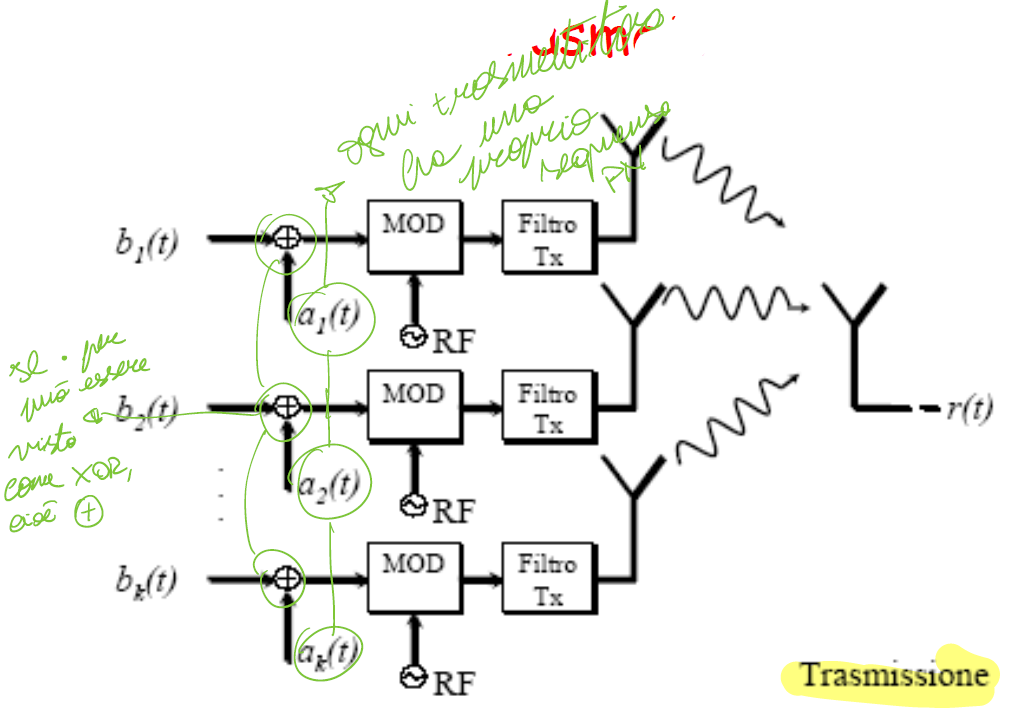
\includegraphics[scale = 0.65]{Trasmissione CDMA.png}
\end{figure}

Di seguito uno schema a blocchi di un ricevitore in cui i trasmettitori applicano il CDMA (con note): 

\begin{figure}[h]
    \centering
    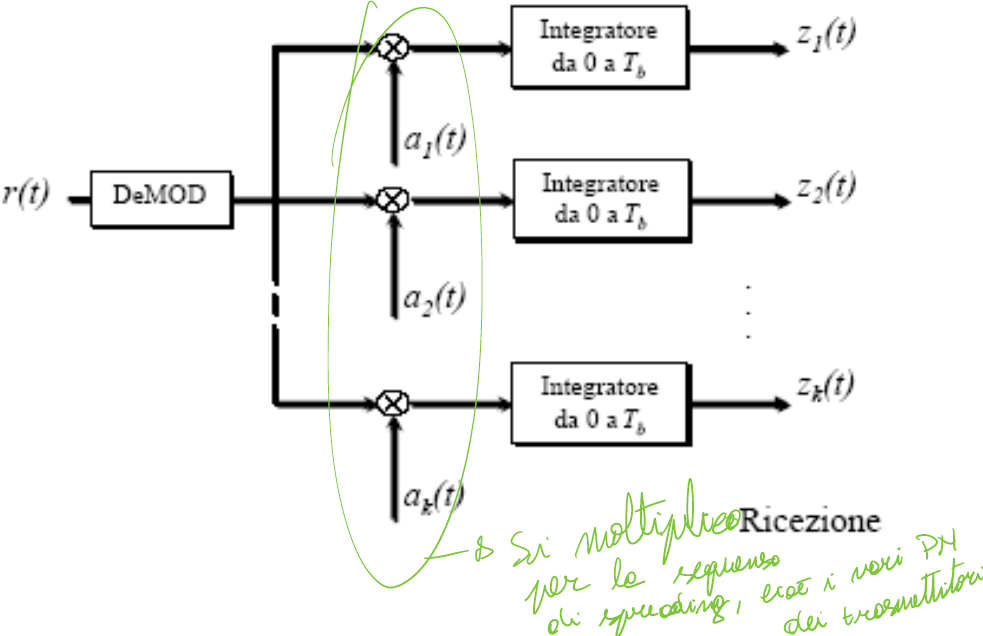
\includegraphics[scale = 0.65]{Ricezione CDMA.png}
\end{figure}

\newpage 

\subsection{CDMA: valutazione più accurata}
\footnote{Slide del prof | Spettro espanso | pag 34 - 36 \\
Appunti di Damiano | pag 34 - 36\\
Slide | Spettro espanso | pag 34 - 36 \\
Appunti | 2025-05-13 | pag 4 - 5
} 

Facendo una valutazione più accurata del segnale in ingresso in CDMA, 
avremo che il segnale r(t) vale: 

{
    \Large 
    \begin{equation}
        r(t)
        =
        \sum_{k = 1}^{N_u}
        \sqrt{2 \cdot P_k}
        \cdot 
        a_k (t - \tau_k)
        \cdot 
        b_k (t - \tau_k)
        \cdot 
        \cos
        \left[
            \gamma_{k} (t)
        \right]
        + 
        n(t)
    \end{equation}
}

dove: 

\begin{itemize}
    \item n(t) sono termini di rumore 
    \item nelle parentesi $(t - \tau_k)$, 
    $\tau_k$ indica il tempo di ritardo del k-esimo trasmettitore 
    perchè i trasmettitori, nel caso reale, non sono sincronizzati allo stesso tempo, 
    e quindi si considera un ritardo 
\end{itemize}

Inoltre, nella formula di r(t) comprare il termine $\gamma_k (t)$ dove: 

{
    \Large 
    \begin{equation}
        \gamma_k (t)
        = 
        \omega_c \cdot (t - \tau_k) + \phi_k
    \end{equation}
}

dove $\phi_k$ è la fase del singolo trasmettitore k-esimo. \newline 

Se consideriamo l'i-esimo utente, abbiamo che: 

{
    \Large 
    \begin{equation}
        \begin{cases}
            \tau_i = 0 
            \\
            \phi_i = 0
        \end{cases}
    \end{equation}
}

La demodulazione si realizza moltiplicando r(t) per d(t): 

{
    \Large 
    \begin{equation}
        d(t)
        =
        \sqrt{2} 
        \cdot
        a_i(t)
        \cdot
        \cos(\omega_c \cdot t)
    \end{equation}
}

Allora possiamo esprimere questa formula: 

{
    \Large 
    \begin{equation}
        \begin{split}
            z_i 
            &=
            r_i \cdot d(t)
            \\
            &=
            \sqrt{P_i} \cdot b_i \cdot \int_{0}^{T_b} a_i^{2} (t) dt 
            \\
            &+ \sum_{k = 1, k \neq i}^{N_u}
            \sqrt{P_k}
            \cdot 
            \int_{0}^{T_b}
            a_k (t - \tau_k)
            \cdot
            b_k (t - \tau_k)
            \cdot 
            a_i (t) 
            \cdot 
            \cos(\phi_k - \omega_c \cdot \tau_k)
            dt 
            \\ 
            &+
            \eta_i (t)
        \end{split} 
    \end{equation}
}

Nella formula di $z_i$, il termine: 

{
    \Large 
    \begin{equation}
    \sqrt{P_i} \cdot b_i \cdot \int_{0}^{T_b} a_i^{2} (t) dt         
    \end{equation}
}

è il termine utile perchè il termine di auto-correlazione. \newline 

Invece, l'altra parte dell'equazione è considerata disturbo. \newline 

In particolare $\eta_i$ è il contributo del rumore termico che può espresso come segue: 

{
    \Large 
    \begin{equation}
        \eta_i 
        = 
        \int_{0}^{T_b} 
        n^{'} (t) \cdot a_i (t) dt
    \end{equation}
}

Se: 

{
    \Large 
    \begin{equation}
        \tau_k = 0
    \end{equation}
}

allora il termine: 

{
    \Large 
    \begin{equation}
        \int_{0}^{T_b}
            a_k (t - \tau_k)
            \cdot
            b_k (t - \tau_k)
            \cdot 
            a_i (t) 
    \end{equation}
}

diventa la correlazione mutua tra $a_k$ e $a_i$. \newline 

Nel CDMA possiamo considerare due scenari. \newline 

Il primo scenario, quello ideale, 
ha le seguenti caratteristiche: 

\begin{itemize}
    \item ritardi uguali per tutti i segnali, quindi:
    {
        \Large
        \begin{equation}
            \tau_k = 0 \text{ per } \forall k
        \end{equation}
    }
    \item fase iniziale nulla per tutti le portanti, quindi: 
    {
        \Large 
        \begin{equation}
            \phi_k = 0
        \end{equation}
    }
\end{itemize}

In questo primo scenario, $z_i$ diventa: 

{
    \Large 
    \begin{equation}
        \begin{split}
        z_i 
        &=
        \sqrt{P_i} \cdot b_i \cdot R_{ii} (0) 
        \\
        &+ 
        \sum_{k = 1}^{N_u}
        \sqrt{P_k} \cdot b_k \cdot R_{ki} (0)
        \\
        &+ 
        \eta_i
        \end{split}
    \end{equation}
}

dove: 

\begin{itemize}
    \item $R_{ii} (0)$ è l'auto-correlazione di $a_i (t)$
    \item $R_{ki} (0)$ è la mutua-correlazione tra $a_k (t)$ e $a_i (t)$
\end{itemize} 

Se ci troviamo nel caso ideale: 

{
    \Large 
    \begin{equation}
        R_{ki} (0) = 0
    \end{equation}
} 

e di conseguenza $z_i$ diventa: 

{
    \Large 
    \begin{equation}
        z_i = \sqrt{P_i} \cdot b_i \cdot R_{ii} (0) + \eta_i
    \end{equation}
}

cioè, in parole, se la mutua-correlazione tra $a_k (t)$ e $a_i (t)$ è nulla, 
allora avremo $z_i$ minimo e potremo ricostruire il messaggio senza problemi. \newline 

Se invece consideriamo il secondo scenario, 
dove si hanno ritardi diversi per i segnali per ogni utente, 
cioè: 

{
    \Large 
    \begin{equation}
        \tau_i \neq \tau_k
    \end{equation}
}

avremo una trasmissione asincrona, 
ad esempio in un caricamento di un radiomobile, 
ad esempio un cellulare, 
verso una stazione radio-base. \newline 

\begin{tcolorbox}
    Un caso storico di tecnologia mobile,  
    al suo fallimento dovuto al ritardo di sincronizzazione e di fase 
    tra la cella radio-base e il dispositivo radiomobile  
    è lo standard WiiMAX, 
    il quale ha perso il successo tecnologico mobile  
    grazie alla migliore implementazione dello standard 4G. \newline 
    
    Il tema è discusso più a fondo in questo video: \newline 

    \url{https://youtu.be/bq7iUaplYbQ?si=X8UFf18bmVDRNsoC} \\ How 4G killed Sprint by Speedify
\end{tcolorbox}

Cioè: 

{
    \Large 
    \begin{equation}
        R_{ki} (\tau_k) \to R_{ki} (0)
    \end{equation}
}

o in inglese, out-of-phase cross-correlation. \newline 

Anche se a priori non conosciamo quanto vale $R_{ki} (\tau_k)$, 
vogliamo che sia la più bassa possibile. \newline 

\newpage 

\subsection{Auto-correlazione, cross-correlazione, sequenza PN, prestazioni CDMA}
\footnote{Slide del prof | Spettro espanso | pag 37 - 40 \\
Appunti di Damiano | pag 37 - 38, 40 \\
Slide | Spettro espanso | pag 37 - 40 \\
Appunti | 2025-05-13 | pag 5 
} 

Come al solito, 
ci sono molto utili i grafici piuttosto che le formule. \newline 

Per esempio una auto-correlazione di una sequenza di lunghezza 31 è la seguente: 

\begin{figure}[h]
    \centering
    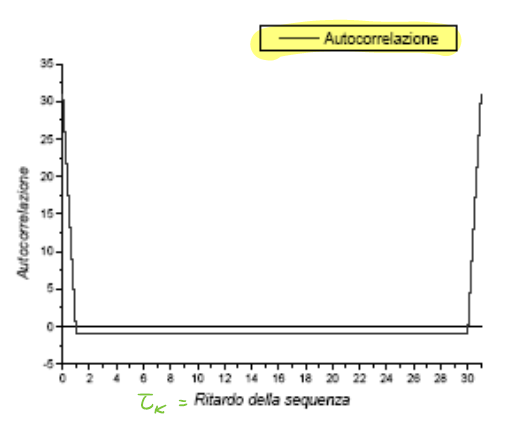
\includegraphics[scale = 0.65]{autocorrelazione di una sequenza di 31 elementi.png}
\end{figure}

Una gold-sequence (ne approfondiremo dopo) di lunghezza 31 ha l'andamento di una mutua correlazione di questo tipo: 

\begin{figure}[h]
    \centering
    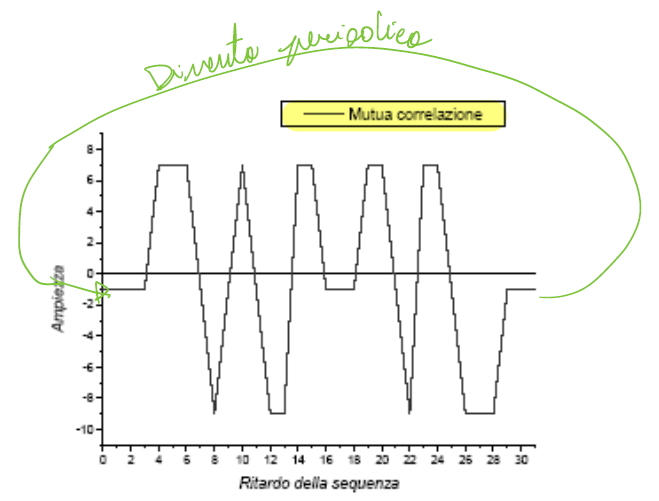
\includegraphics[scale = 0.65]{Mutua correlazione di una gold sequenza di lunghezza 31.png}
\end{figure}

Una gold sequence PN ha questo andamento: 

\begin{figure}[h]
    \centering
    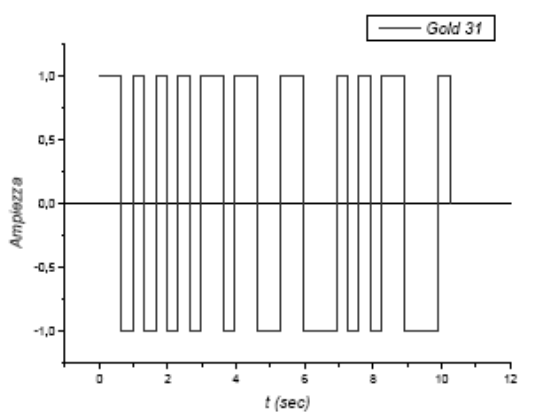
\includegraphics[scale = 0.65]{gold sequenza di lunghezza 31.png}
\end{figure}

\newpage 

Un andamento della prestazione del BER rispetto al numero di utenti K, 
e l'SNR, che nel caso digitale è $\frac{E_b}{N_0}$, è il seguente: 

\begin{figure}[h]
    \centering
    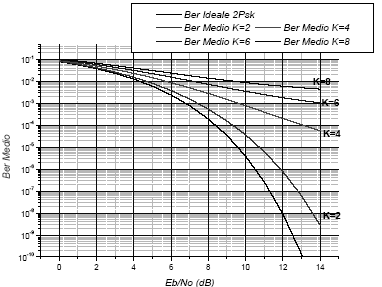
\includegraphics[scale = 1.5]{BER in CDMA con K utenti grafico.png}
\end{figure}

Come si può notare, 
all'aumentare degli utenti K, 
il BER peggiora (la curva si trova più in alto). \newline 

\newpage

\subsection{Communications over multipath channels}
\footnote{Slide del prof | Spettro espanso | pag 41 \\
Slide | Spettro espanso | pag 41 \\
Appunti | 2025-05-13 | pag 6 
} 

Come il caso precedente della valutazione della CDMA, 
nella DS-SS bisogna considerare anche le comunicazioni lungo 
percorsi multipli, dall'inglese multipath channels. \newline 

Possiamo considerare due scenari su questi percorsi multipli per una DS-SS: 

\begin{enumerate}
    \item utente singolo 
    \item multi-utente
\end{enumerate}

Considerando il primo caso, 
cioè il singolo utente, 
possiamo modellare il segnale ricevuto r(t) in DS-SS come: 

{
    \Large 
    \begin{equation}
        r(t)
        = 
        a(t) \cdot b(t) \cos(\omega_c \cdot t)
        + 
        \sum_{i = 1}^{L}
        A_i 
        \cdot 
        a(t - \tau_i)
        \cdot 
        b(t - \tau_i)
        \cos(\gamma_i (t))
        + 
        n(t)
    \end{equation}
}

Nella formula di r(t), 
il termine: 

{
    \Large 
    \begin{equation}
        \sum_{i = 1}^{L}
        A_i 
        \cdot 
        a(t - \tau_i)
        \cdot 
        b(t - \tau_i)
        \cos(\gamma_i (t))
        + 
        n(t)
    \end{equation}
}

dove con L si indicano le L repliche del segnale $a(t) \cdot b(t) \cos(\omega_c \cdot t)$ 
dovute dai percorsi multipli. \newline 

Al ricevitore è presente un integratore e quindi riceveremo il segnale z: 

{
    \Large 
    \begin{equation}
        z 
        = 
        b \cdot R_{SS} (0)
        + 
        \sum_{i = 1}^{L}
        A_i 
        \cdot
        \int_{0}^{T_b} 
        a(t - \tau_i)
        \cdot 
        b(t - \tau_i)
        \cos(\gamma_i (t))
        + 
        \eta(t)
    \end{equation}
}

Invece, nel secondo caso, cioè in caso di comunicazione in percorsi multipli con diversi utenti, 
occorre tener conto degli altri segnali interferenti, 
ciascuno con il proprio insieme di cammini multipli. \newline 

La modellazione matematica sarebbe più complicata da svolgere rispetto al caso del singolo utente. \newline 

\newpage 

\subsection{Pulsed interference}
\footnote{Slide del prof | Spettro espanso | pag 42 - 43\\
Appunti di Damiano | pag 42 - 43\\
Slide | Spettro espanso | pag 42 - 43 \\
Appunti | 2025-05-13 | pag 6 - 7
} 

Si definisce pulsed interference un segnale interferente a burst (nel tempo), 
con spettro di  potenza piatto nell'intera banda di trasmissione (in frequenza). \newline 

\begin{tcolorbox}
    Ricordiamo bene la relazione tra tempo e frequenza dal vecchio corso.
\end{tcolorbox}

La differenza tra un disturbo a banda larga generico, 
e un disturbo burst sta nel suo tempo, che ha un carattere "impulsato". \newline 

L'interferenza di tipo impulsato, realmente, disturba un pacchetto di bit. \newline 

Andando più a fondo nella trattazione matematica, 
se indichiamo con il carattere $\beta$ la percentuale di tempo per cui l'interferente 
disturba la trasmissione, 
se $P_I$ è la potenza media trasmessa, 
negli intervalli di disturbo "impulsato", 
la potenza dell'interferente diventa $P_I^{'}$:

{
    \Large 
    \begin{equation}
        P_I^{'}
        = 
        \frac{P_I}{\beta}
    \end{equation}
}

In presenza di solo disturbo impulsato, 
quindi non considerando rumore termico o altre cause di disturbo, 
possiamo calcolarci la probabilità di errore sul bit $P_{Eb}$ che vale: 

{
    \Large 
    \begin{equation}
        P_{Eb}
        = 
        Q 
        \left(
            \sqrt{\frac{2 \cdot E_b}{\frac{I_0}{\beta}}}
        \right)
    \end{equation}
}

Questa formula di $P_{Eb}$ è valida quando l'interferente è attivo. \newline 

Come visto nei precedenti capitoli, con Q si intende di calcolarci l'erfc dell'argomento di Q. \newline 

\newpage 

\subsubsection{Pulsed interference: worst case scenario}
\footnote{Slide del prof | Spettro espanso | pag 44 \\
Appunti di Damiano | pag 44 \\
Slide | Spettro espanso | pag 44 \\
Appunti | 2025-05-13 | pag 7 
} 

Dalla formula di probabilità di errore media è: 

{
    \Large 
    \begin{equation}
        P_{Eb}
        =
        \beta
        \cdot
           Q 
        \left(
            \sqrt{\frac{2 \cdot E_b}{\frac{I_0}{\beta}}}
        \right)
    \end{equation}
}

\begin{tcolorbox}
Se poniamo $\beta = 1$ nella formula di $P_{Eb}$, ricaviamo la formula di trasmissione in DS-SS con solo rumore termico    
\end{tcolorbox}

Derivando questa formula (senza fare la secondo derivata), 
cioè:

{
    \Large 
    \begin{equation}
        \frac{\partial P_{Eb}}{\partial \beta}
        = 
        0
    \end{equation}
}

possiamo trovare il valore $\beta^{*}$ che massimizza la funzione $P_{Eb}$ media. \newline 

Quindi, senza fare i calcoli, 
possiamo scrivere che $\beta^{*}$ vale: 

{
    \Large 
    \begin{equation}
        \beta^{*}
        = 
        \begin{cases}
            \frac{0.71}{\frac{E_b}{I_0}} \text{ per } \frac{E_b}{I_0} \ge 0.71 
            \\
            1 \text{ per } \frac{E_b}{I_0} \le 0.71
        \end{cases}
    \end{equation}
}

Mettendo il valore di $\beta^{*}$ in $P_{Eb}$, 
possiamo ricavarci $\left. P_{Eb} \right|_{max}$ come: 

{
    \Large 
    \begin{equation}
        \left. P_{Eb} \right|_{max}
        = 
        \begin{cases}
            \frac{0.082}{\frac{E_b}{I_0}} \text{ per } \frac{E_b}{I_0} \ge 0.71 
            \\
            Q 
        \left(
            \sqrt{\frac{2 \cdot E_b}{I_0}}
        \right) \text{ per } \frac{E_b}{I_0} \le 0.71
        \end{cases}
    \end{equation}
}

\newpage 

\subsubsection{Pulsed interference: prestazioni}
\footnote{Slide del prof | Spettro espanso | pag 45 \\
Appunti di Damiano | pag 45 \\
Slide | Spettro espanso | pag 45 \\
Appunti | 2025-05-13 | pag 7 
} 

Sapendo la formula media di $P_{Eb}$ è: 

{
    \Large 
    \begin{equation}
          P_{Eb}
        =
        \beta
        \cdot
           Q 
        \left(
            \sqrt{\frac{2 \cdot E_b}{\frac{I_0}{\beta}}}
        \right)
    \end{equation}
}

possiamo metterla in relazione con il rapporto segnale-rumore, 
cioè in digitale $\frac{E_b}{I_0}$. \newline 

In base al valore di $\beta$, 
possiamo tracciare il seguente grafico per confrontare le prestazioni delle pulsed intereference: 

\begin{figure}[h]
    \centering
    \includegraphics[scale = 0.7]{Probabilità di errore e SNR in segnali burst.png}
\end{figure}

La retta tratteggiata in figura è proprio la formula che avevamo trovato precedentemente, 
cioè: 

{
    \Large 
    \begin{equation}
         \left. P_{Eb} \right|_{max}
         = 
         \frac{0.082}{\frac{E_b}{I_0}} \text{ per } \frac{E_b}{I_0} \ge 0.71 
    \end{equation}
}

Dal seguente grafico possiamo svolgere due considerazioni riguardo al caso peggiore: 

\begin{itemize}
    \item la penalizzazione può essere molto rilevante 
    \item l'uso di un FEC (Forward Error Correction, cioè un algoritmo di correzione in cui non si chiede la ritrasmissione del segnale) classico, non risolve il problema  
\end{itemize}

\newpage 

\subsubsection{Pulsed interference: miglioramento delle prestazioni tramite interlever}
\footnote{Slide del prof | Spettro espanso | pag 46 - 47\\
Appunti di Damiano | pag 46 - 47\\ 
Slide | Spettro espanso | pag 46 - 47 \\
Appunti | 2025-05-13 | pag 7 - 8
} 


Siccome, in questi casi peggiori, non possiamo usare i FEC, 
allora si è pensato di usare l'interlever (in italiano permutatore) per migliore la trasmissione. \newline 

Uno schema di una trasmissione DS-SS con interlever al trasmettitore e de-interlever al ricevitore 
è il seguente (con note): 

\begin{figure}[h]
    \centering
    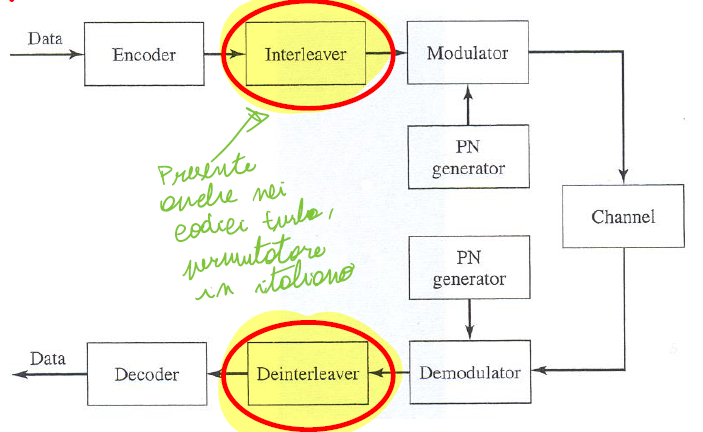
\includegraphics[scale = 1]{Interleveler e deinterleveler per migliorare la trasmissione.png}
\end{figure}

Da un punto di vista grafico, con un esempio di 4 utenti, 
possiamo descrivere il funzionamento dell'interlever, che opera righe per colonne, 
con il seguente schema (con note): 

\begin{figure}[h]
    \centering
    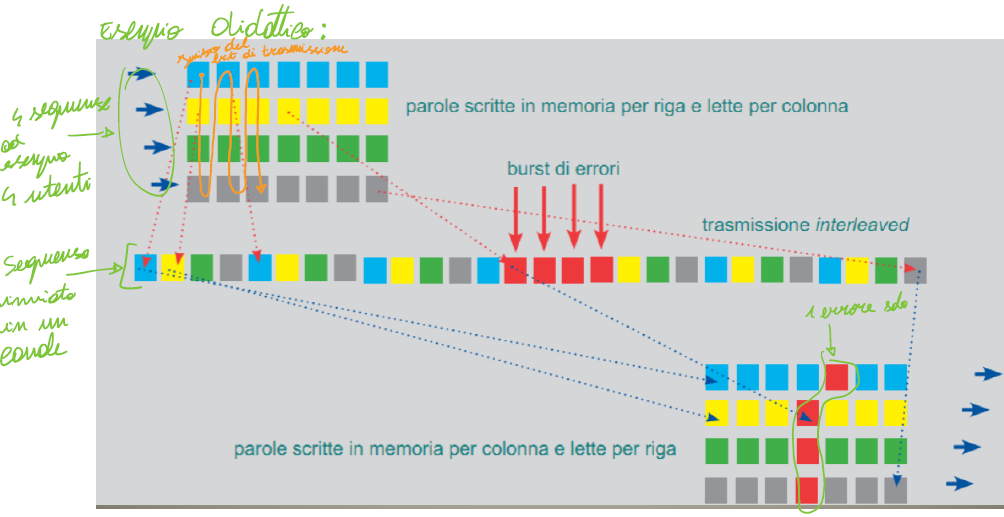
\includegraphics[scale = 0.85]{Funzionamento interleveler esempio.png}
\end{figure}

Come si vede dalla figura, 
a causa del rumore burst, 
avremo solo un errore di bit per ogni utente, 
quindi l'errore viene "distribuito". \newline 

Ma, il problema è che questo "mischiamento" ha bisogno di tempo e aggiunge ritardo al sistema, 
specialmente se abbiamo a che fare con delle matrici molto grandi. \newline 

\newpage 

\section{Generazione di sequenze PN}
\footnote{Slide del prof | Spettro espanso | pag 48 \\
Appunti | 2025-05-16 | pag 1 
} 

\begin{tcolorbox}
Un piccolo ripasso del PN con LFSR, 
ma approfondiremo un aspetto molto importante che vedrete poi    
\end{tcolorbox}

Una sequenza pseudo-random o pseudo-noise (PN) 
è una sequenza binaria in cui la proprietà di correlazione è simile 
(per quanto possibile) a quella del rumore bianco. \newline 

\newpage 

\subsection{Maximum-length sequences (m-sequences)}
\footnote{Slide del prof | Spettro espanso | pag 49 - 51\\
Appunti di Damiano | pag 49 - 50\\
Appunti | 2025-05-16 | pag 1 
} 

Dal precedente capitolo, 
sappiamo che che una generazione di una sequenza può essere svolta con un LFSR (Linear Feedback Shift Register), 
il quale ha una lunghezza L massima pari a: 

{
    \Large 
    \begin{equation}
        L = 2^{m} - 1
    \end{equation}
}

Uno schema di un LFSR per la generazione di PN è la sequenza (con note): 

\begin{figure}[h]
    \centering
    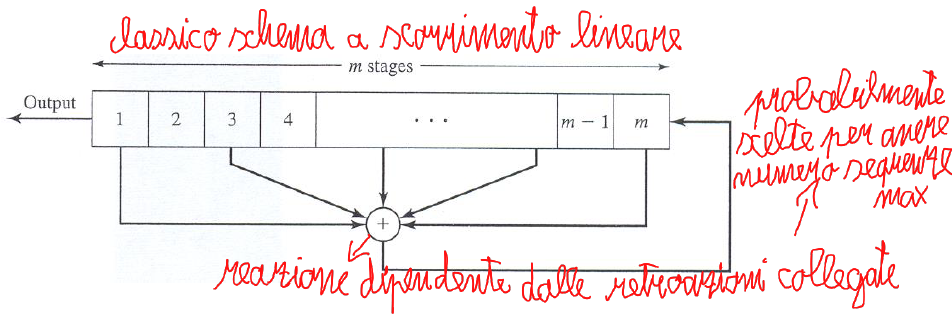
\includegraphics[scale = 0.8]{LFSR per PN con note.png}
\end{figure}

Il LFSR è inizializzato con un valore qualsiasi 
che prende il nome di seme (o seed in inglese) 
purché diverso da zero. \newline 

Per ogni m ci sono più possibilità di collegamento retro-azionati. \newline 

Di seguito un esempio per ogni m: 

\begin{figure}[h]
    \centering
    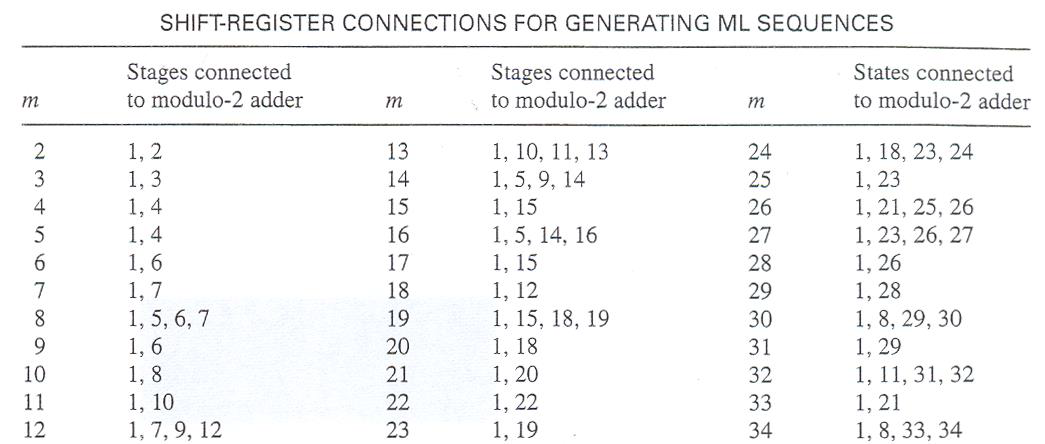
\includegraphics[scale = 0.8]{sequenze m tabella LFSR.png}
\end{figure}

La sequenza prodotta dall'LFSR è, 
originariamente, una sequenza di 0 e 1. \newline 

Ai fini dell'utilizzo nel sistema DS-SS, 
la sequenza viene convertita in una sequenza di coefficiente $\{ c_n\}$ in cui il singolo elemento $c_n$ diventa: 

{
    \Large 
    \begin{equation}
        \begin{cases}
            c_n = 0 \to c_n = - 1 
            \\
            c_n = 1 \to c_n = 1
        \end{cases}
    \end{equation}
}

Come studiato nel capitolo precedente, 
siccome siamo nel valore dei discreti $\mathbb{Z}_{2}$, 
la funzione di auto-correlazione $R_c (m)$ non sarà un integrale, 
bensì una sommatoria esprimibile come: 

{
    \Large 
    \begin{equation}
        R_c (m)
        = 
        \sum_{n = 1}^{L}
        c_n \cdot c_{n+m} \text{ per } 0 \le m \le L-1
    \end{equation}
}

Anche la funzione di auto-correlazione $R_c (m)$ 
è periodica di periodo L. \newline 

\newpage 

\subsubsection{Proprietà delle m-sequences}
\footnote{Slide del prof | Spettro espanso | pag 52 \\
Appunti di Damiano | pag 52 \\
Appunti | 2025-05-16 | pag 1 
} 

La sequenza PN ideale dovrebbe avere: 

{
    \Large 
    \begin{equation}
        R_C (m) 
        = 
        \begin{cases}
            L \text{ per } m = 0
            \\
            0 \text{ per } 1 \le m \le L-1
        \end{cases}
    \end{equation}
}

Invece nelle m-sequenze l'auto-correlazione $R_C (m)$ 
è uguale a: 

{
    \Large 
    \begin{equation}
        R_C (m) 
        = 
        \begin{cases}
            L \text{ per } m = 0
            \\
            -1 \text{ per } 1 \le m \le L-1
        \end{cases}
    \end{equation}
}



Se facciamo il rapporto tra l'autocorrelazione e la correlazione, 
calcoliamo la cross-correlazione, che vale: 

{
    \Large 
    \begin{equation}
        \frac{R_C (m)}{R_C (0)} =  - \frac{1}{L}
    \end{equation}
}

Se L tende ad infinito, il rapporto diventa: 

{
    \Large
    \begin{equation}
      \frac{R_C (m)}{R_C (0)} \to 0 \text{ per }  L \to + \infty  
    \end{equation}
}

\newpage 

\subsection{Cross-correlazione}
\footnote{Slide del prof | Spettro espanso | pag 53 \\
Appunti di Damiano | pag 53 \\
Appunti | 2025-05-16 | pag 1 - 2 
} 

Come sempre detto, 
generalmente si useranno le seguenti tabelle (con note): 

\begin{figure}[h]
    \centering
    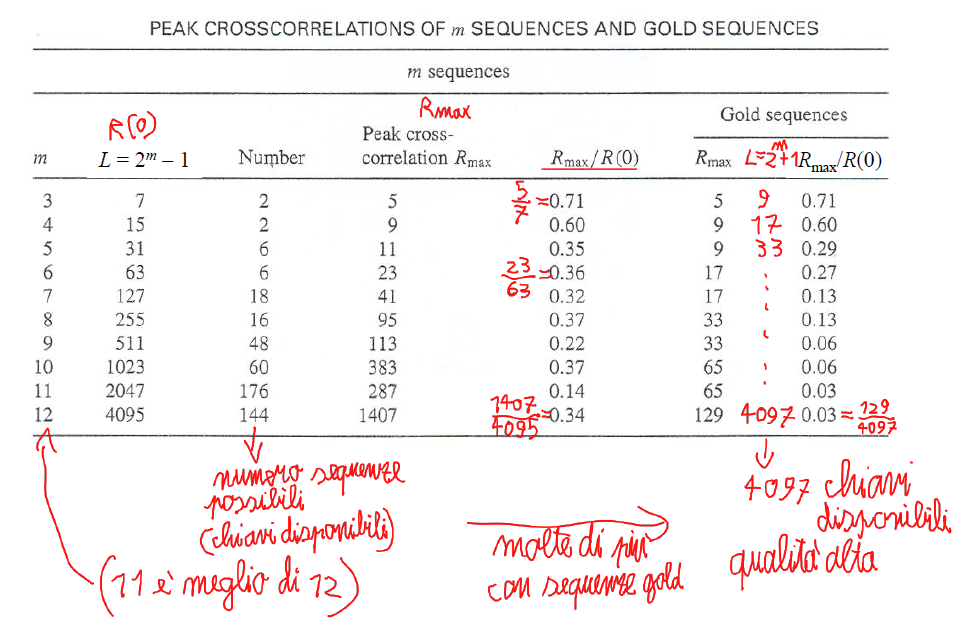
\includegraphics[scale = 0.8]{cross-correlazione tabella.png}
\end{figure}

All'aumentare di m, 
il rapporto $\frac{R_{max}}{R(0)}$ non decresce: ha un andamento altalenante. \newline 

Nella tabella qui in figura, $\frac{R_{max}}{R(0)}$ è troppo alto. \newline 

Nel DS-SS si vuole avere un $\frac{R_{max}}{R(0)}$ più bassa possibile: 
per risolvere questo problema vengono usate le gold-sequence. \newline 

Se $\frac{R_{max}}{R(0)}$, si possono servire più utenti nel CDMA. \newline 

\newpage 

\section{Gold-sequences}
\footnote{Slide del prof | Spettro espanso | pag 57 - 61 \\
Appunti di Damiano | pag 57 - 60\\
Appunti | 2025-05-16 | pag 3 - 4
} 

Le gold-sequences sono quelle sequenze che sono ottenute a partire da una coppia selezionata di m-sequenze, 
e formando le somme modulo 2 per ognuna delle L versioni shiftate di una sequenza rispetto all'altra. \newline 

Di seguito un esempio di una sequenza gold (con note): 

\begin{figure}[h]
    \centering
    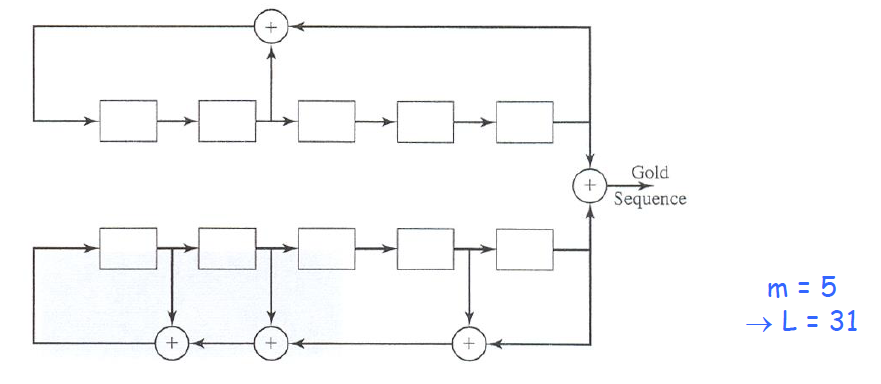
\includegraphics[scale = 0.8]{sequenza gold con m = 5.png}
\end{figure}

Per generare una sequenza gold, 
bisogna partire da una condizione iniziale, diversa da zero, 
nel primo generatore. \newline 

Si ottengono $2^{m}$ sequenze di gold cambiando il seme del secondo generatore, 
da 0 a L, in cui: 

{
    \Large 
    \begin{equation}
        L = 2^{m} - 1
    \end{equation}
}

Questo è equivalente a dire che si fa partire il secondo generatore da una di $2^{m}$ 
diverse condizioni iniziali. \newline 

Un'ultima sequenza di Gold è quella fornita dal secondo generatore da solo, 
ottenuta ponendo a zero il seme del primo generatore. \newline  

In totale si hanno $2^{m} + 1$ sequenze di Gold. \newline 

Nelle sequenze di Gold, 
si possono avere 3 valori possibili di cross-correlazione: 

\begin{itemize}
    \item -1 
    \item - t(m) 
    \item t(m) - 2
\end{itemize}

dove t(m) è la massima cross-correlazione: può essere indicata anche con $R_{max}$. \newline 

t(m) può avere due tipi di valori in base alla scelta di m: 

{
    \Large 
    \begin{equation}
        t(m)
        =
        \begin{cases}
            2^{\frac{m+1}{2}} + 1 \text{ per m dispari} 
            \\ 
            2^{\frac{m+2}{2}} + 1 \text{ per m dispari}
        \end{cases}
    \end{equation}
}

Siccome bisogna sempre progettare il caso peggiore, 
bisogna prendere il caso peggiore, che è t(m) con m pari. \newline 

Ricordiamo che il numero massimo delle sequenze è L + 2. \newline 

Per m dispari e sufficientemente grande, $R_{max}$ vale: 

{
    \Large 
    \begin{equation}
        \begin{split}
            R_{max} 
            &= 
            \sqrt{2^{m+1}} + 1 
            \\
            &\approx 
            \sqrt{2 \cdot 2^{m}}
            \\
            &\approx
            \sqrt{2 \cdot L}
        \end{split}
    \end{equation}
}

Se invece m è pari e sufficientemente grande, $R_{max}$ vale: 

{
    \Large 
    \begin{equation}
        \begin{split}
            R_{max} 
            &= 
            \sqrt{2^{m+2}} + 1 
            \\
            &\approx 
            \sqrt{2^{2} \cdot 2^{m}}
            \\
            &\approx
            2 \cdot \sqrt{ L}
        \end{split}
    \end{equation}
}

\newpage 

\section{Lower bound}
\footnote{Slide del prof | Spettro espanso | pag 62 \\
Appunti di Damiano | pag 62 \\
Appunti | 2025-05-16 | pag 5 
} 

Per aumentare gli utenti, ad esempio nel CDMA DS-SS, 
oltre alle sequenze gold, 
sono presenti alti tipi di sequenze per massimizzare $\frac{R_{max}}{R(0)}$. \newline 

Per un insieme di N sequenze di periodo L, 
il matematico Welch definì il Welch bound, cioè un valore minimo possibile teorico di $R_{max}$, 
che vale: 

{
    \Large
    \begin{equation}
        R_{max}
        \geq 
        L \cdot \sqrt{\frac{N -1}{N \cdot L - 1}}
    \end{equation}
}

Quando N è sufficientemente grande, 
la formula precedente diventa: 

{
    \Large
    \begin{equation}
        \begin{split}
        R_{max}
        &\geq 
        L \cdot \sqrt{\frac{N -1}{N \cdot L - 1}}
        \\
        &\downarrow
        \\
        R_{max}
        &\geq 
        \sqrt{L} \text{ per } N >> 1
        \end{split}
    \end{equation}
}

Confrontando l'$R_{max}$ con quello 
che si può ottenere con le sequenze gold: 

{
    \Large 
    \begin{equation}
        R_{max} \ge \sqrt{2 \cdot L}
    \end{equation}
}

se si vuole massimizzare i clienti e si considera come parametro solo $R_{max}$, 
meglio prendere le sequenze di Welch che hanno un $R_{max}$ minore. \newline 

Le sequenze di Gold si definiscono sub-ottime (significa che si può fare di meglio). \newline 

Invece altri sequenze, come quella di Kasami, sono definite ottime perchè hanno: 

{
    \Large 
    \begin{equation}
        R_{max}
        \approx
        \sqrt{L}
    \end{equation}
}

\newpage 

\section{Kasami sequences (small set)}
\footnote{Slide del prof | Spettro espanso | pag 63 - 64\\
Appunti di Damiano | pag 63 - 64\\
Appunti | 2025-05-16 | pag 5 - 6
} 

Le sequenze Kasami sono definite ottime perchè hanno: 

{
    \Large 
    \begin{equation}
        R_{max}
        \approx
        \sqrt{L}
    \end{equation}
}

In altri termini, 
si utilizzano le sequence Kasami per ottenere valori minimi di cross-correlazione, 
cioè $R_{max}$. \newline 

Possiamo definire due tipi di sequenze Kasami: 

\begin{itemize}
    \item small set 
    \item Large set
\end{itemize}

Adesso andiamo ad analizzare le sequenze Kasami small set. \newline 

Uno schema su come si ottengono le sequenze Kasami (con note): 

\begin{figure}[h]
    \centering
    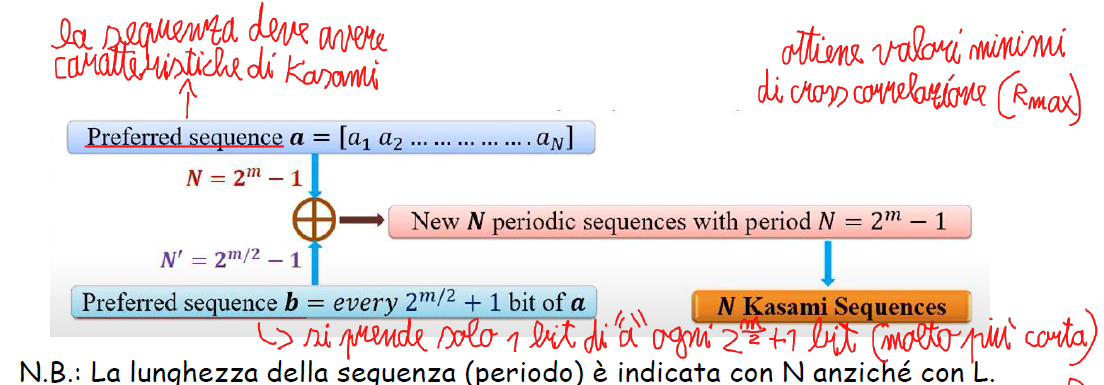
\includegraphics[scale = 0.8]{Sequenze Kasami small set con note.png}
\end{figure}

Dalle sequenze Kasami si hanno N sequenze, 
dove N vale: 

{
    \Large 
    \begin{equation}
        N = 2^{\frac{m}{2}}
    \end{equation}
} 

A parità di m, 
come le sequenze gold,  
le sequenze Kasami sono minori rispetto a quelle gold. \newline 

Cioè si passa dalle $2^{m} - 1$ sequenze delle gold alle $2^{\frac{m}{2}}$ delle Kasami. \newline 

Come illustrato dallo schema, 
le sequenze Kasami sono ottenute considerando due vettori $\overrightarrow{a}$ e $\overrightarrow{b}$ 
e tutte le versioni traslate di $\overrightarrow{b}$, 
che ha periodo $2^{\frac{m}{2}} - 1$, quindi $2^{\frac{m}{2} - 2}$. \newline 

\begin{tcolorbox}
    Vettori e sequenze vengono utilizzati come sinonimi, 
    perchè, come ben sai dai corsi di programmazione, 
    un computer o un microcontrollore non riescono ad interpretare un vettore come un qualcosa di fisico, 
    bensì il vettore viene interpretato come una sequenza di bit. 
\end{tcolorbox}

Andando a fondo, 
la sequenza $\overrightarrow{b}$ viene ottenuta per "decimazione" 
delle sequenza $\overrightarrow{a}$, 
selezionando un bit ogni $2^{\frac{m}{2}} + 1 $ bit di $\overline{a}$. \newline 

$\overrightarrow{b}$ è periodica e di periodo $2^{\frac{m}{2}} - 1$. \newline 

Ogni periodo di $\overrightarrow{a}$ include $2^{\frac{m}{2}} + 1$ periodi di $\overrightarrow{b}$. \newline 

Inoltre, per costruire le sequenze Kasami, m deve essere pari. \newline 

La funzione di cross-correlazione assume 3 valori: 

\begin{itemize}
    \item -t 
    \item -1 
    \item t - 2
\end{itemize}


dove t vale: 

{
    \Large 
    \begin{equation}
        t = 2^{\frac{m}{2}} + 1
    \end{equation}
}

\newpage 

\section{Kasami sequences (large set)}
\footnote{Slide del prof | Spettro espanso | pag 66 - 68\\
Appunti di Damiano | pag 66 - 68\\
Appunti | 2025-05-16 | pag 6 
} 

Un esempio di schema di sequenze Kasami large-set è il seguente: 

\begin{figure}[h]
    \centering
    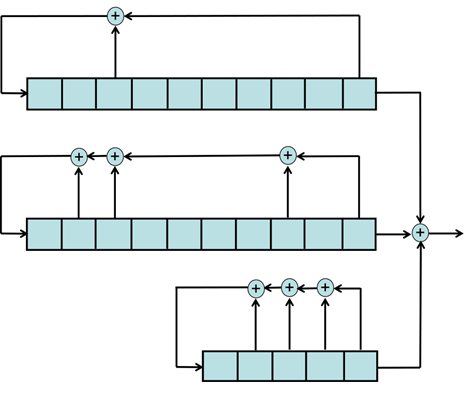
\includegraphics[scale = 0.8]{Sequenze Kasami large set.png}
\end{figure}

In questo caso, 
al posto delle small set, 
si utilizzano due sequenze preferite, 
e la versione decimata di una di queste. \newline 

La versione decimata deve essere di lunghezza: 

{
    \Large 
    \begin{equation}
        \text{mod }
        (m, 4) = 2
    \end{equation}
}

Ad esempio, m = 2 è un valore possibile da utilizzare. \newline 

Il periodo L è come quello delle small set:

{
    \Large
    \begin{equation}
        L = 2^{m} - 1
    \end{equation}
}

Invece il numero di sequenze N è diverso, 
cioè:

{
    \Large 
    \begin{equation}
        N = 2^{\frac{3 \cdot m}{2}} + 2^{\frac{m}{2}} 
    \end{equation}
}

La funzione di cross-correlazione assume questi 5 valori: 

\begin{itemize}
    \item - t 
    \item -s 
    \item -1 
    \item s - 2 
    \item t - 2  
\end{itemize}

dove: 

{
    \Large 
    \begin{equation}
        \begin{cases}
        t = 2^{\frac{m}{2 + 1}} + 1 
        \\
        s = \frac{t + 1}{2}
        \end{cases}
    \end{equation}
}

$R_{max}$ che si ottiene con le sequenze Kasami large set è un valore maggiore rispetto alle small set. \newline 

\newpage 

\section{Sequenze di Barker}
\footnote{Slide del prof | Spettro espanso | pag 69 - 71\\
Appunti di Damiano | pag 69\\
Appunti | 2025-05-16 | pag 7 
} 

Una caratteristica principale delle sequenze utilizzate fino adesso 
è stato l'auto-correlazione periodica. \newline 

Invece le sequenze di Barker sono sequenze che hanno un'auto-correlazione aperiodica. \newline

Nello specifico, 
definita la funzione di auto-correlazione aperiodica di una sequenza bipolare $\{ b_j\}$, 
dove $j = 1, \dots, L$ come: 

{
    \Large 
    \begin{equation}
        C_k = \sum_{j = 1}^{L-K} b_j \cdot b_{j+k} \text{ per } k = 0, \dots, L-1
     \end{equation}
}

\begin{tcolorbox}
Come scritto precedente, 
l'auto-correlazione periodica è diversa rispetto all'auto-correlazione aperiodica; 
questo lo si può notare anche dalle sommatorie impiegate. \newline 

Useremo $\sum_{j = 1}^{L-K}$ per l'auto-correlazione aperiodica, 
invece $\sum_{j = 1}^{L}$ per l'auto-correlazione periodica. 
\end{tcolorbox}

Una sequenza, o codice, di Barker verifica la proprietà: 

{
    \Large 
    \begin{equation}
        \abs{C_k} \le 1 \text{ per } \forall k \neq 0
    \end{equation}
}

Inoltre, non esistono codici di Barker con $L > 13$. \newline 

Esempi di utilizzi di sequenze di Barker sono: 

\begin{itemize}
    \item come prefisso per il recupero del sincronismo di una trama 
    \item come sequenza di speading nell'IEEE 802.11b, cioè il Wi-Fi 1 adottato nel 1999, se L = 11
\end{itemize}

\newpage 

\section{Frequency-Hopping Spread-Spectrum (FH-SS)}
\footnote{Slide del prof | Spettro espanso | pag 72 - 75\\
Appunti di Damiano | pag 72 - 73\\
Appunti | 2025-05-16 | pag 8 
} 

La FH-SS è una tecnologia usata principalmente nell'ambito militare. \newline 

La banda disponibile W è divisa in un certo numero elevato di slot di frequenze distinte. \newline 

Nella trasmissione dell'n-esimo simbolo, 
si utilizza uno o più di questi slot. \newline 

Gli slot vengono selezionati in modo pseudo-random, 
sulla base dell'uscita di un generatore PN. \newline 

Oppure, spiegato in altri termini, 
il trasmettitore salta da una banda all'altra secondo regole pseudo-casuali. \newline 

Solo chi è a conoscenza della sequenza pseudo-causale tra una frequenza all'altra può ricevere il segnale. \newline 

Chi intercetta una porzione del segnale poi non sa dove si troverò lo stesso segnale in un secondo momento. \newline 

Di seguito uno schema di trasmissione e ricezione in FH-SS (con note):  

\begin{figure}[h]
    \centering
    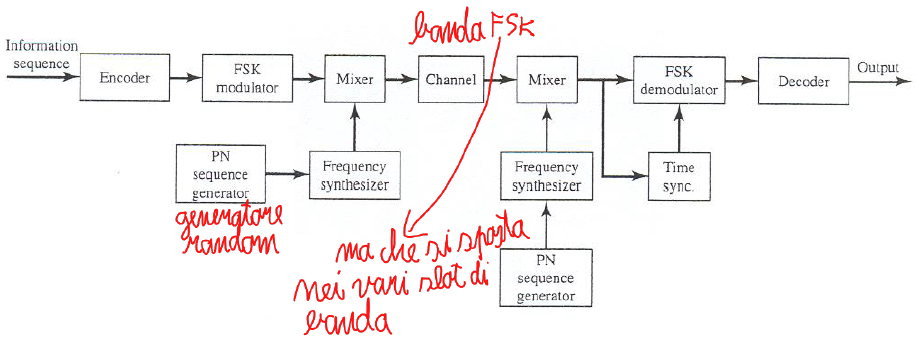
\includegraphics[scale = 0.8]{FH-SS schema a blocchi.png}
\end{figure}

Generalmente la modulazione utilizzata nell'FH-SS è M-FSK. \newline 

La frequenza in uscita dal modulatore FSK viene traslata in ragione dell'uscita del sintetizzatore di frequenza. \newline 

\newpage 

Di seguito un grafico di una trasmissione FH-SS 
in cui viene indicata la frequenza utilizzata lungo il tempo: 

\begin{figure}[h]
    \centering
    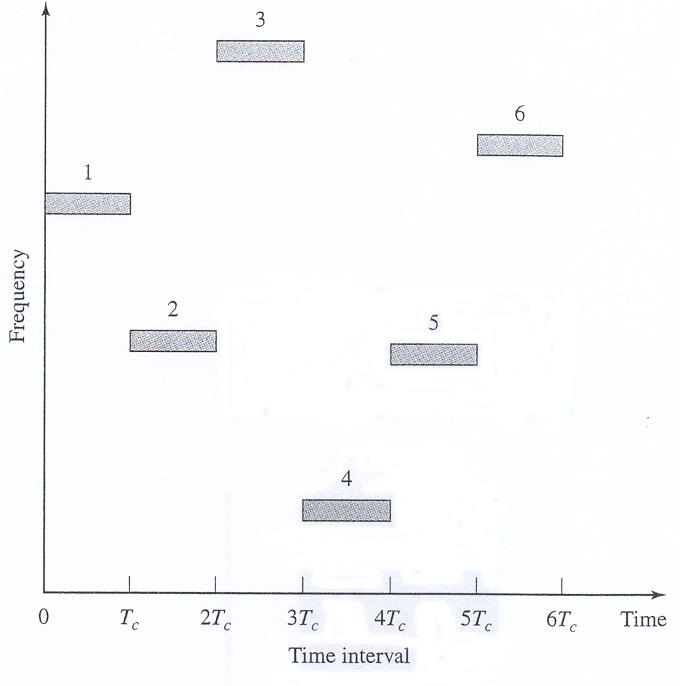
\includegraphics[scale = 0.6]{FH-SS frequenza utilizzata nel tempo.png}
\end{figure}

oppure un altro grafico di FH-SS: 

\begin{figure}[h]
    \centering
    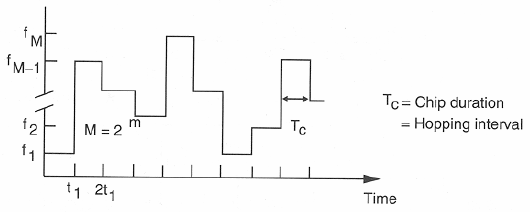
\includegraphics[scale = 1]{FH-SS frequenza utilizzata nel tempo secondo grafico.png}
\end{figure}

Rispetto alle figure, l'intervallo di Hopping non verrà indicato come $T_c$, 
bensì con $T_H$. \newline 

I vantaggi della FH-SS sono le seguenti: 

\begin{itemize}
    \item minori problemi di sincronizzazioni 
    \item guadagni di processo più elevati rispetto alla DS-SS 
    \item notevole immunità al jamming intenzionale
\end{itemize}


\newpage 

\subsection{Classificazione dei sistemi FH-SS}
\footnote{Slide del prof | Spettro espanso | pag 76 \\
Appunti di Damiano | pag 76 \\
Appunti | 2025-05-16 | pag 8 
} 

I sistemi FH-SS si possono classificare in: 

\begin{itemize}
    \item SFH, o Slow Frequency Hopping 
    \item FFH, o Fast Frequency Hopping 
    \item IFH, o Intermediate Frequency Hopping
\end{itemize}

La loro classificazione dipende dal periodi di Hopping $T_H$ 
rispetto al periodo di bit $T_b$. \newline 

Si definisce una SF quando: 

{
    \Large 
    \begin{equation}
        T_H > T_b
    \end{equation}
}

o, visto in dal punto di vista del tasso (o rate in inglese): 

{
    \Large 
    \begin{equation}
        R_H < R_b
    \end{equation}
}

Andando più nel dettaglio, 
nel periodo di tempo fra due portanti vengono generati più bit, 
cioè, sulla stessa portante vengono trasmesse sequenze di alcuni o molti bit 
(in certe implementazioni vengono trasmessi più di 1000 bit nella stessa frequenza). \newline 

Si definisce una FFH quando: 

{
    \Large 
    \begin{equation}
        \begin{split}
            T_H &< T_b
            \\
            &\updownarrow
            \\
            R_H &> R_b
        \end{split}
    \end{equation}
}

La frequenza di portante cambia più volte durante la trasmissione di un bit, 
alche la FFH è largamente diffusa per scopi militari. \newline 

In altri termini, per trasmettere un bit viene diviso in più più frequenze. \newline 

Alla fine, possiamo definire l'ultima FH-SS che è la IFH, 
in cui:

{
    \Large 
    \begin{equation}
        \begin{split}
            T_H &\approx T_b
            \\
            &\updownarrow
            \\
            R_H &\approx R_b
        \end{split}
    \end{equation}
}

\newpage 

FINE PROGRAMMA A.A. 2024/2025 \newline 

BUON ESAME !!!


\begin{figure}[h]
    \centering
    
\includegraphics[scale = 0.4]{meme.jpg}
\end{figure}
